\documentclass[slug=SZ, room=Hermann-Krone-Bau\,\ Labor\ 1.25, supervisor=Martin\ Kroll]{../../Lab_Report_LaTeX/lab_report}

\title{Solarzelle}
\author{Oliver Matthes, Valentin Boettcher}
\usepackage[version=4]{mhchem}
\usepackage{todonotes}
\graphicspath{ {figs/} }
\newcommand{\sun}[1]{\SI{#1}{Sonne}}
\newcommand{\mwcm}[1]{\SI{#1}{\milli\watt\per\centi\meter^2}}
\newcommand{\voc}{V_{\text{OC}}}
\newcommand{\isc}{I_{\text{SC}}}
\newcommand{\jsc}{j_{\text{SC}}}
\usepackage{circuitikz}
\usepackage{subcaption}
\usepackage{ amssymb }
\usepackage{tabularx}
\sisetup{math-celsius = {}^{\circ}\kern-\scriptspace C}
\usepackage[ngerman]{babel}

% bib
\addbibresource{protokoll.bib}

\begin{document}
\maketitle

\section{Einleitung}
\label{sec:einl}

Die Energiegewinnung aus erneuerbaren Energien spielt eine entscheidende Rolle, wenn es darum geht,
aus der Energieproduktion mittels fossiler Energieträger auszusteigen.
Auch Solarzellen steuern dazu einen wichtigen Beitrag bei. Deswegen ist es wichtig, diese
Technologie weiterzuentwickeln.

Solarzellen wandeln durch Lichtabsorption Strahlung in elektrische Energie um (photovoltaischer Effekt).
Dafür müssen Solarzellen die eintreffende Strahlung natürlich absorbieren.
Außerdem muss es aufgrund dieser Absorption zu einer Anregung von beweglichen Ladungsträgern
(positiven und negativen) kommen, die von einander getrennt werden müssen.

Zur Erfüllung dieser Kriterien, benötigt man einen Übergang zwischen zwei verschieden dotierten
Halbleitern (p-n-Übergang, vgl.~\ref{sec:pnüber}).

\subsection{Halbleiter}
\label{sec:halbleiter}

Die beste Erklärung der elektrischen Eigenschaften von Halbleitern liefert das Bändermodell.
Dieses Modell besteht aus Energiebändern und Bandlücken.

In einem einzelnem Atom können Elektronen nur diskrete Energiewerte annehmen.
Kristalle allerdings bestehen aus sehr vielen Atomen (\(\approx 10^{23}\)), mit einem geringen Abstand zu einander,
der dazu führt, dass die Wellenfunktionen der Elektronen überlappen und somit die Energieniveaus in sehr
viele Unterniveaus aufspalten, die praktisch kontinuierlich aussehen.
Zwischen diesen Energiebändern befinden sich Bandlücken, die einen nicht erlaubten Bereich darstellen und
einen Abstand \(E_g\) besitzen.

Das bei einer Temperatur von  \(T=0 K\)  höchste vollbesetzte Band nennt man das \emph{Valenzband}.
Die maximale Energie, die die Elektronen bei \(T=0 K\) besitzen \emph{Fermienergie}. Das nächst höhere Band ist
also nicht vollständig besetzt, weswegen sich Ladungsträger ziemlich gut auf diesem fortbewegen können, da
ihnen viele unbesetzte Zustände zur Verfügung stehen.
Aufgrund dieser Eigenschaft wird jenes Band als \emph{Leitungsband} bezeichnet.
Um ein Elektron also aus dem Valenz- in das Leitungsband anzuheben, muss es die Bandlücke überqueren,
wofür es genügend Energie benötigt. Diese erhält es durch die Absorption von Strahlung der Energie:

\begin{equation}\label{eq:bandenenergie}
        E_g = h\nu
\end{equation}

Bei einer Temperatur von \(T=0 K\) sind Halbleiter ebenso wie Isolatoren nichtleitend.
Der Unterschied zwischen den Beiden ist die Größe der Bandlücke. Diese ist bei Isolatoren relativ groß,
bei Halbleitern hingegen eher klein, sodass schon geringe Energien ausreichen, um Elektronen aus dem Valenz-
in das Leitungsband anzuheben.

Der Unterschied zwischen den beiden ist die Größe der Bandlücke. Diese ist bei Isolatoren relativ groß,
bei Halbleitern hingegen eher klein, sodass schon geringe Energien ausreichen, um Elektronen aus dem Valenz-
in das Leitungsband anzuheben.

\subsection{Dotierung von Halbleitern}
\label{sec:dotierung}

Unter Dotierung versteht man die "Verunreinigung" des eigentlichen Halbleitermaterials mit Fremdatomen, um
die Eigenschaften dieses Halbleiters zu verändern.
Man unterscheidet dabei zwischen \emph{n-dotierten Halbleitern} und \emph{p-dotierten Halbleitern}.

\begin{description}

        \item[n-dotierte Halbleiter]
        Bringt man in einen Siliziumkristall, dessen Atome je vier Valenzelektronen
        besitzen, ein paar Atome, die beispielsweise fünf Valenzelektronen (z.B. Phosphor) haben, so binden die
        vier Siliziumelektronen vier der Elektronen der Fremdatome. Ein Außenelektron es Phosphors bleibt also
        ungebunden und dient als Ladungsträger. Die nun positiv geladenen Phosphoratome sitzen fest im Kristall,
        können sich also nicht bewegen und dienen deswegen nicht als Ladungsträger.
        Da thermisch angeregte Elektron-Loch-Paare in dotierten Halbleitern relativ selten vorkommen und die
        beweglichen Elektronen der Hauptladungsträger sind, nennt man diese \emph{Majoritätsladungsträger}, die
        Elektron-Loch-Paare entsprechend \emph{Minoritätsladungsträger}.

        \item[p-dotierte Halbleiter]
        Bei p-dotierten Halbleitern macht man genau das Gegenteil von dem, was man
        bei den n-dotierten getan hat. Statt Fremdatome mit fünf bringt man solche mit drei Valenzelektronen
        in den Siliziumkristall ein. Das nun fehlende Elektron steuert das Silizium bei. Dadurch entsteht eine
        frei bewegliche positive Ladung, ein so genanntes Loch, das jetzt den \emph{Majoritätsladungsträger}
        darstellt.

\end{description}

Durch die Dotierung kommt es zu einem Ladungsträgerungleichgewicht, das die Fermie-Energie in Richtung des
Majoritätsladungsträger enthaltenden Bandes.

\subsection{p-n-Übergang von Halbleitern}
\label{sec:pnüber}

Ein p-n-Übergang findet statt, wenn man einen p-dotierten und einen n-dotierten Halbleiter in Kontakt miteinander
bringt. Im n-Gebiet befinden sich mehr Elektronen als im p-Gebiet. Dadurch kommt es zu einem Konzentrationsgefälle
und die Löcher diffundieren Richtung n-Gebiet, die Elektronen Richtung p-Gebiet. Treffen beide Ladungsträger
aufeinander rekombinieren sie. Aufgrund dessen sinkt die Zahl der Ladungsträger nahe der Grenze der beiden
Halbleiter und es entsteht eine so genannte \emph{Verarmungszone}. Die Atome, mit denen der Halbleiter
dotiert worden ist, sind, wie in \ref{sec:dotierung} unbeweglich. Deswegen bleiben diese in der Verarmungszone
zurück und es entsteht ein negativ geladener Bereich im p-dotierten und ein positiv geladener im
n-dotierten Halbleiter. Diese beiden Bereiche zusammen werden als \emph{Raumladungszone} bezeichnet.
In dieser Zone entsteht also durch diese festen Ladungen eine Potentialdifferenz, die der Diffusion der
beweglichen Ladungen entgegen wirkt. Im Gleichgewicht zwischen Diffusion und Feldstrom ist die
\emph{Raumladungszone} gleich der \emph{Verarmungszone}.\\

Unter Anlegung einer äußeren Spannung verhält sich der p-n-Übergang wie eine Diode, d.h. es gibt eine Sperr-
und eine Durchlassrichtung.
Setzt man den Minuspol an das n-Gebiet und den Pluspol entsprechend an den p-Halbleiter, dann ist die Spannung
in Durchlassrichtung gepolt. Die Elektronen im n-Gebiet werden vom Minuspol abgestoßen und in die Raumladungszone
gedrückt. Äquivalentes passiert mit den Löchern im p-Gebiet. Dadurch wird ein Stromfluss ermöglicht.
Legt man die Pole entgegengesetzt an die Diode an, bewegen sich die Elektronen des n-Gebiets logischerweise in
Richtung des positiven Pols, die Löcher entsprechend gen Minuspol auf der anderen Seite. Dadurch wird die
Raumladungszone vergrößert und es fehlen Ladungsträger, um einen Stromfluss zu ermöglichen.

Dieses Verhalten einer idealen Diode wird durch ihre Kennlinie beschrieben, die mit der \emph{Shockley-Gleichung}
dargestellt werden kann.

\begin{equation}\label{eq:shockley}
        I = I_S \cdot \qty(\exp[\frac{eU}{a \cdot k_B T}]-1)
\end{equation}

\begin{tabular}{llll}
         & \(I_S\) & ... & Sättigungsstrom        \\
         & \(a\)   & ... & Diodenidealitätsfaktor \\
         & \(k_B\) & ... & Boltzmann-Konstante    \\
         & \(T\)   & ... & Temperatur
\end{tabular}

\newpage

Mit

\begin{equation}\label{eq:sattigstrom}
        I_S = I_{S0} \cdot \exp[-\frac{E_g}{k_B T}]
\end{equation}

\begin{tabular}{lllllll}
         & \(I_{S0}\) & ... & Sättigungsstrom bei \(T=0 K\) &
\end{tabular}

\subsection{Lichtabsorption in Halbleitern}
\label{sec:absorp}

Um Strom erzeugen zu können, müssen Solarzellen das auf sie einstrahlende Licht absorbieren.
Diese Eigenschaft wird durch das Absorptionsgesetz beschrieben:

\begin{equation}\label{eq:absorp}
        i(z) = (1-R) \cdot i_0 \cdot \exp[-\alpha x]
\end{equation}

\begin{tabular}{llll}
         & \(i\)      & ... & transmittierte Lichtintensität bei Materialdurchgang Richtung x \\
         & \(R\)      & ... & Reflektivität                                                   \\
         & \(i_0\)    & ... & einfallende Strahlintensität                                    \\
         & \(\alpha\) & ... & Absorptionskoeffizient
\end{tabular}\\ \\

Dabei sollte die Absorption möglichst groß sein. Dafür muss \(i\) möglichst klein werden, was bedeutet, dass
\(\alpha\) und \(x\) recht groß sein sollten.\\

Um nutzbar absorbiert werden zu können, müssen die Photonen eine Mindestenergie besitzen, damit die Elektronen
die Bandlücke überwinden können (vgl.~\ref{eq:bandenenergie}). Wenn die Photonen allerdings mehr Energie als
die Größe der Bandlücke besitzen, geht die überschüssige Energie der Ladungsträger durch Relaxation an die
Bandkanten verloren. Die Größe der Bandlücke bestimmt also die Energie, die pro Photon, das absorbiert wurde,
genutzt werden kann.

\subsubsection{Direkte und indirekte Halbleiter}
\label{sec:dirindhalb}

Wenn das Minimum des Leitungsbandes und das Maximum des Valenzbandes im Impulsraum gegeneinander verschoben sind,
muss zusätzlich zur Absorption eines Photons ein Impuls durch die Wechselwirkung mit einem Phonon aufgenommen
werden. Man spricht in diesem Fall von indirekten Halbleitern. Die Interaktion zwischen drei Teilchen ist
allerdings recht unwahrscheinlich verglichen mit direkten Halbleitern, bei denen die Aufnahme eines Photons schon
ausreichend ist.
Deswegen müssen Solarzellen aus indirekten Halbleitern, wie zum Beispiel Silizium, wesentlich dicker als die
aus direkten (z. B. Galliumarsenid) sein.

\subsection{Funktionsweise einer Solarzelle}
\label{sec:solar}

Wird eine Solarzelle beleuchtet, entstehen dann durch die Photonenabsorption Elektron-Loch-Paare. Falls diese in der
Raumladungszone entstehen, werden die entgegengesetzten Ladungen der Paare durch die Raumladung in der
Verarmungszone von einander getrennt:
Die Elektronen werden Richtung n-Gebiet gezogen, die positiv geladenen Löcher gen p-Gebiet.
Erreichen die Ladungsträger das Ende der Raumladungszone so treiben sie die anderen gleichnamigen Ladungsträger
vor sich her und es entsteht eine Spannung. Ist ein Verbraucher angeschlossen, so fließt durch diesen der so genannte \emph{Photostrom}.
Erfolgt die Photonenabsorption und damit die Ladungsträgerpaarerzeugung nicht innerhalb der Verarmungszone,
müssen diese Paare erst durch den Halbleiter in diese Zone diffundieren.

\subsubsection{Ersatzschaltbild}
\label{sec:ersatz}

Geht man von einer idealen Solarzelle aus, so kann man diese als Diode auffassen. Ein Generator sorgt dabei
im Ersatzschaltbild für den Photostrom, der durch Beleuchtung der Solarzelle entsteht. Um die in einer
Solarzelle auftretenden Verluste darzustellen, nutzt man einerseits einen Serienwiderstand für den
Bahnwiderstand des Materials des Halbleiters und der Kontakte sowie einen Parallelwiderstand, der die an einer
nicht idealen p-n-Grenzfläche auftretende Leckströme beschreibt.
Damit folgt für den Gesamtstrom einer Solarzelle:

\begin{equation}\label{eq:ersatz}
        I = I_{Ph} - I_S \cdot \qty(\exp[\frac{e(U-IR_S)}{a \cdot k_B T}] -1 ) - \frac{U-IR_S}{R_P}
\end{equation}

\begin{tabular}{llll}
         & \(I_{Ph}\) & ... & Photostrom                   \\
         & \(I_S\)    & ... & Sättigungsstrom              \\
         & \(U\)      & ... & von außen angelegte Spannung \\
         & \(R_S\)    & ... & Serienwiderstand             \\
         & \(R_P\)    & ... & Parallelwiderstand
\end{tabular}\\ \\

Das Ersatzschaltbild ergibt sich zu:

\begin{figure}[h]\centering
  \label{fig:schaltbild}
  \begin{circuitikz}
    \draw
    (0,0) to[european current source] (0,2.5)
    to node[currarrow, rotate=90]{} (0,2) node[right]{\(I_{Ph}\)}
    to [short] (0, 2.5) to [short] (1.5, 2.5)
    to node[currarrow, rotate=-90] {} (1.5,2) node[right]{\(I_D\)}
    to[stroke diode] (1.5, .5)
    to[short] (1.5, 0) to[short] (0, 0);
    \draw
    (1.5,2.5) to [short] (3,2.5)
    to[european resistor, l=$R_P$] (3, 0)
    to [short] (1.5,0);
    \draw
    (3,2.5) to [european resistor, l=\(R_S\)] (5,2.5)
    to node[currarrow] {} (5.5,2.5) node[above]{\(I\)};
    \draw
    (3,0) to [short] (5.5,0);
    \draw
    [-latex](5,2) -- (5,.5) node[right]{\(U\)};
  \end{circuitikz}
  \caption{Ersatzschaltbild einer Solarzelle.}
\end{figure}

\subsubsection{Kennlinie der Solarzelle}

Ist die Solarzelle unbeleuchtet so gleicht ihre Kennlinie der einer Diode.
Der Kennlinie der beleuchteten Zelle kann man einiges entnehmen.
Zum einen die Leerlaufspannung \(\voc\), also die Spannung für \(I=0 A\), den Kurzschlussstrom \(I_{SC}\), der den
Strom darstellt, der fließt, wenn keine äußere Spannung anliegt und den maximalen Leistungspunkt, also der Punkt
der maximalen Leistung der Solarzelle. Außerdem findet man mit dem Füllfaktor \emph{FF}, der sich aus dem
Quotienten von maximaler Leistung und \(|I_{SC}| \cdot \voc\) bestimmt, den Wirkungsgrad der Zelle:

\begin{equation}\label{eq:wirkgrad}
        \eta = \frac{FF \cdot |\isc| \cdot \voc}{P_{ein}}
\end{equation}

\begin{tabular}{llll}
         & \(P_{ein}\) & ... & einfallende Strahlungsleistung
\end{tabular}

\subsection{Organische Solarzellen}
\label{sec:orgsolar}

Organische Solarzellen bestehen, wie der Name schon sagt, aus organischen Materialien, was den größten
Unterschied zwischen ihnen und anorganischen ausmacht.
Das organische Material bringt allerdings auch andere Eigenschaften mit, die zu neuen Herausforderungen, aber
auch Vorteilen führen.\\

Eine sehr wichtige neue Eigenschaft ist die kleine Dielektrizitätszahl, die dazu führt, dass sich die durch
Photonenabsorption erzeugten Elektron-Loch-Paare nicht frei bewegen können sondern an dem Molekül, an dem sie
erzeugt wurden, lokalisiert sind. Diesen (angeregten) Zustand des Moleküls nennt man \emph{Exziton}.
Die Trennung der Ladungsträger erfolgt mit Hilfe eines so genannten \emph{Heteroübergangs} wofür man allerdings
ein anderes Molekül benötigt. Das Elektron wird dabei auf dem Elektronenakzeptormaterial zu den Kontakten
abtransportiert die Löcher auf dem Elektronendonatormaterial.
Die Exzitonen werden allein mittels Diffusion durch das Material geleitet. Allerdings besitzen sie nur eine
geringe Diffusionslänge. Damit Exzitonen also noch innerhalb ihrer Lebensdauer, also bevor sie rekombinieren
zu einem Heteroübergang gelangen können, sollte die Strecke, die sie bis zu diesem Übergang zurücklegen müssen,
möglichst gering sein. Aufgrund dessen mischt man die beiden Moleküle miteinander.
Um einen guten Abtransport der getrennten Ladungsträger gewährleisten zu können, sorgt man dafür, dass es in der
Mischschicht der beiden benötigten Moleküle geschlossene Pfade gibt. Gäbe es keine geschlossenen Pfade, könnte
es zu einem recht großen Rekombinationsverlust während des Transport kommen, da sich Elektronen und Löcher
treffen.
Der Vorteil dieser Eigenschaft ist, dass sie, in Kombination mit einem sehr großen Absorptionskoeffizienten
vieler organischer Stoffe in für uns wichtigen Wellenlängenbereichen, sehr dünne Schichten der Solarzellen
ermöglicht.
Ein weiterer großer Vorteil organischer Solarzellen ist ihre Flexibilität, die einen weiten Anwendungsbereich
vor allem im alltäglichen Leben, eröffnet.\\

Ein Nachteil, der allerdings momentan Gegenstand aktueller Forschung ist, ist der noch recht geringe
Wirkungsgrad im Vergleich mit anorganischen Zellen.


\section{Durchf\"uhrung}
\label{sec:durchf}

Nach der Einweisung in den Aufbau und die Inbetriebnahme des Selbigen
wurde die Beleuchtung zun\"achst auf $\sun{1}=\mwcm{1}$
kalibriert. Dies entsprach ungef\"ahr dem verf\"ugbaren Maximum.

Bei der Messung der Leerlaufspannung der Referenzzelle ergibt sich eine
gesch\"atzter Abweichung (untere Grenze) von:

\begin{equation}
  \label{eq:deltavocref}
  \Delta U = \SI{2}{\milli\volt}
\end{equation}

aus der Anzeigegenauigkeit des Multimeters (\SI{1}{\milli\volt}) und
der gesch\"atzten Intensit\"atschwankung durch Inhomogenit\"aten und
Restlicht aus dem Raum (Fenster, Beleuchtung).\\

In dem Versuch wurden folgende Geräte verwendet:

\begin{list}{\(\cdot\)}{}
        \item Keithley 2400 Source Meter
        \item Voltcraft VC130
        \item Halogenbeleuchtung
        \item Temperaturfühler
        \item Lüfter
        \item Computer zur Aufnahme der Messkurven
\end{list}

\todo{ref auf Fehlerrechnung}

\subsection{Vergleich verschiedener Solarzellen-Typen}
\label{sec:vgltyp}

Es wurden f\"ur die in~\ref{tab:atemps} aufgef\"uhrten Solarzellen
jeweils Dunkel und Hellkennlinien aufgenommen. Bei der Aufnahme der
Dunkelkennlinien wurden die Solarzellen zus\"atzlich mit Stoff
abgedeckt.

\begin{table}[h]
  \centering
  \begin{tabular}{ll|SS}
    \toprule
    Zelle & Kurzname & {Temperatur Dunkelkennlinie [\si{\degreeCelsius}]} & {Temperatur
                                                      Hellkennlinie [\si{\degreeCelsius}]}
    \\
    \midrule
    Anorganisch (8) & A8 & 32 & 45 \\
    Organisch & O1 & 26 & 33 \\
    Folie & O2 & 26 & 40 \\
  \end{tabular}
  \caption{Mittlere Temperaturen der Solarzellen.}
  \label{tab:atemps}
\end{table}

\subsection{Einfluss der Beleuchtungsintensit\"at}
\label{sec:einfint}

Es wurde f\"ur f\"unf Intensit\"aten jeweils eine \(I(V)\) Kennlinie
aufgenommen. Die niedrigste Intensität wurde so gew\"ahlt, dass die
Intensit\"at der Halogenbeleuchtung die Umgebungshelligkeit noch
deutlich \"ubertraf und \(\voc\) der Referenzzelle konstant blieb. Das
Maximum wurde zu \(\sun{1}\) gew\"ahlt (siehe~\ref{tab:brefvolts}).

\begin{table}[h]
  \centering
  \begin{tabular}{S}
    \toprule
    {\(\voc\) Referenzzelle [\si{\milli\volt}]}
    \\
    \midrule
    11 \\
    17 \\
    21 \\
    26 \\
    32
  \end{tabular}
  \caption{Lehrlaufspannung der Referenzelle.}
  \label{tab:brefvolts}
\end{table}

\subsection{Solarmodul – Versuche an realistischen Verschaltungen}
\label{sec:solmod}

Es wurde die Beleuchtungsintensit\"at auf der gesamten Fl\"ache des
Aufbaus auf \(\sun{1/3}\) eingestellt, wobei sich durch die
Inhomogenit\"at der Beleuchtung an den R\"andern des Aufbaus
Abweichungen von bis zu \SI{5}{\milli\volt} ergaben. \todo{ref,
  begruendung der Unbedenklichkeit.}

\subsubsection{Solarmodul aus 6 Zellen}
\label{sec:sol6}

Es wurden wurden jeweils zwei Zellen parallelgeschaltet. Drei dieser
Parallelschaltungen wurden dann in Reihe geschaltet und es wurde eine
Hellkennlinie aufgenommen. Diese Bauweise balancierte Robustheit durch
Parallelschaltung und Leistungssteigerung durch Erh\"ohung von
\(\voc\) und \(\isc\) zugleich. (Außerdem sollte \(\isc\)
\SI{1}{\ampere} nicht \"ubersteigen.)

\begin{figure}[H]\centering
  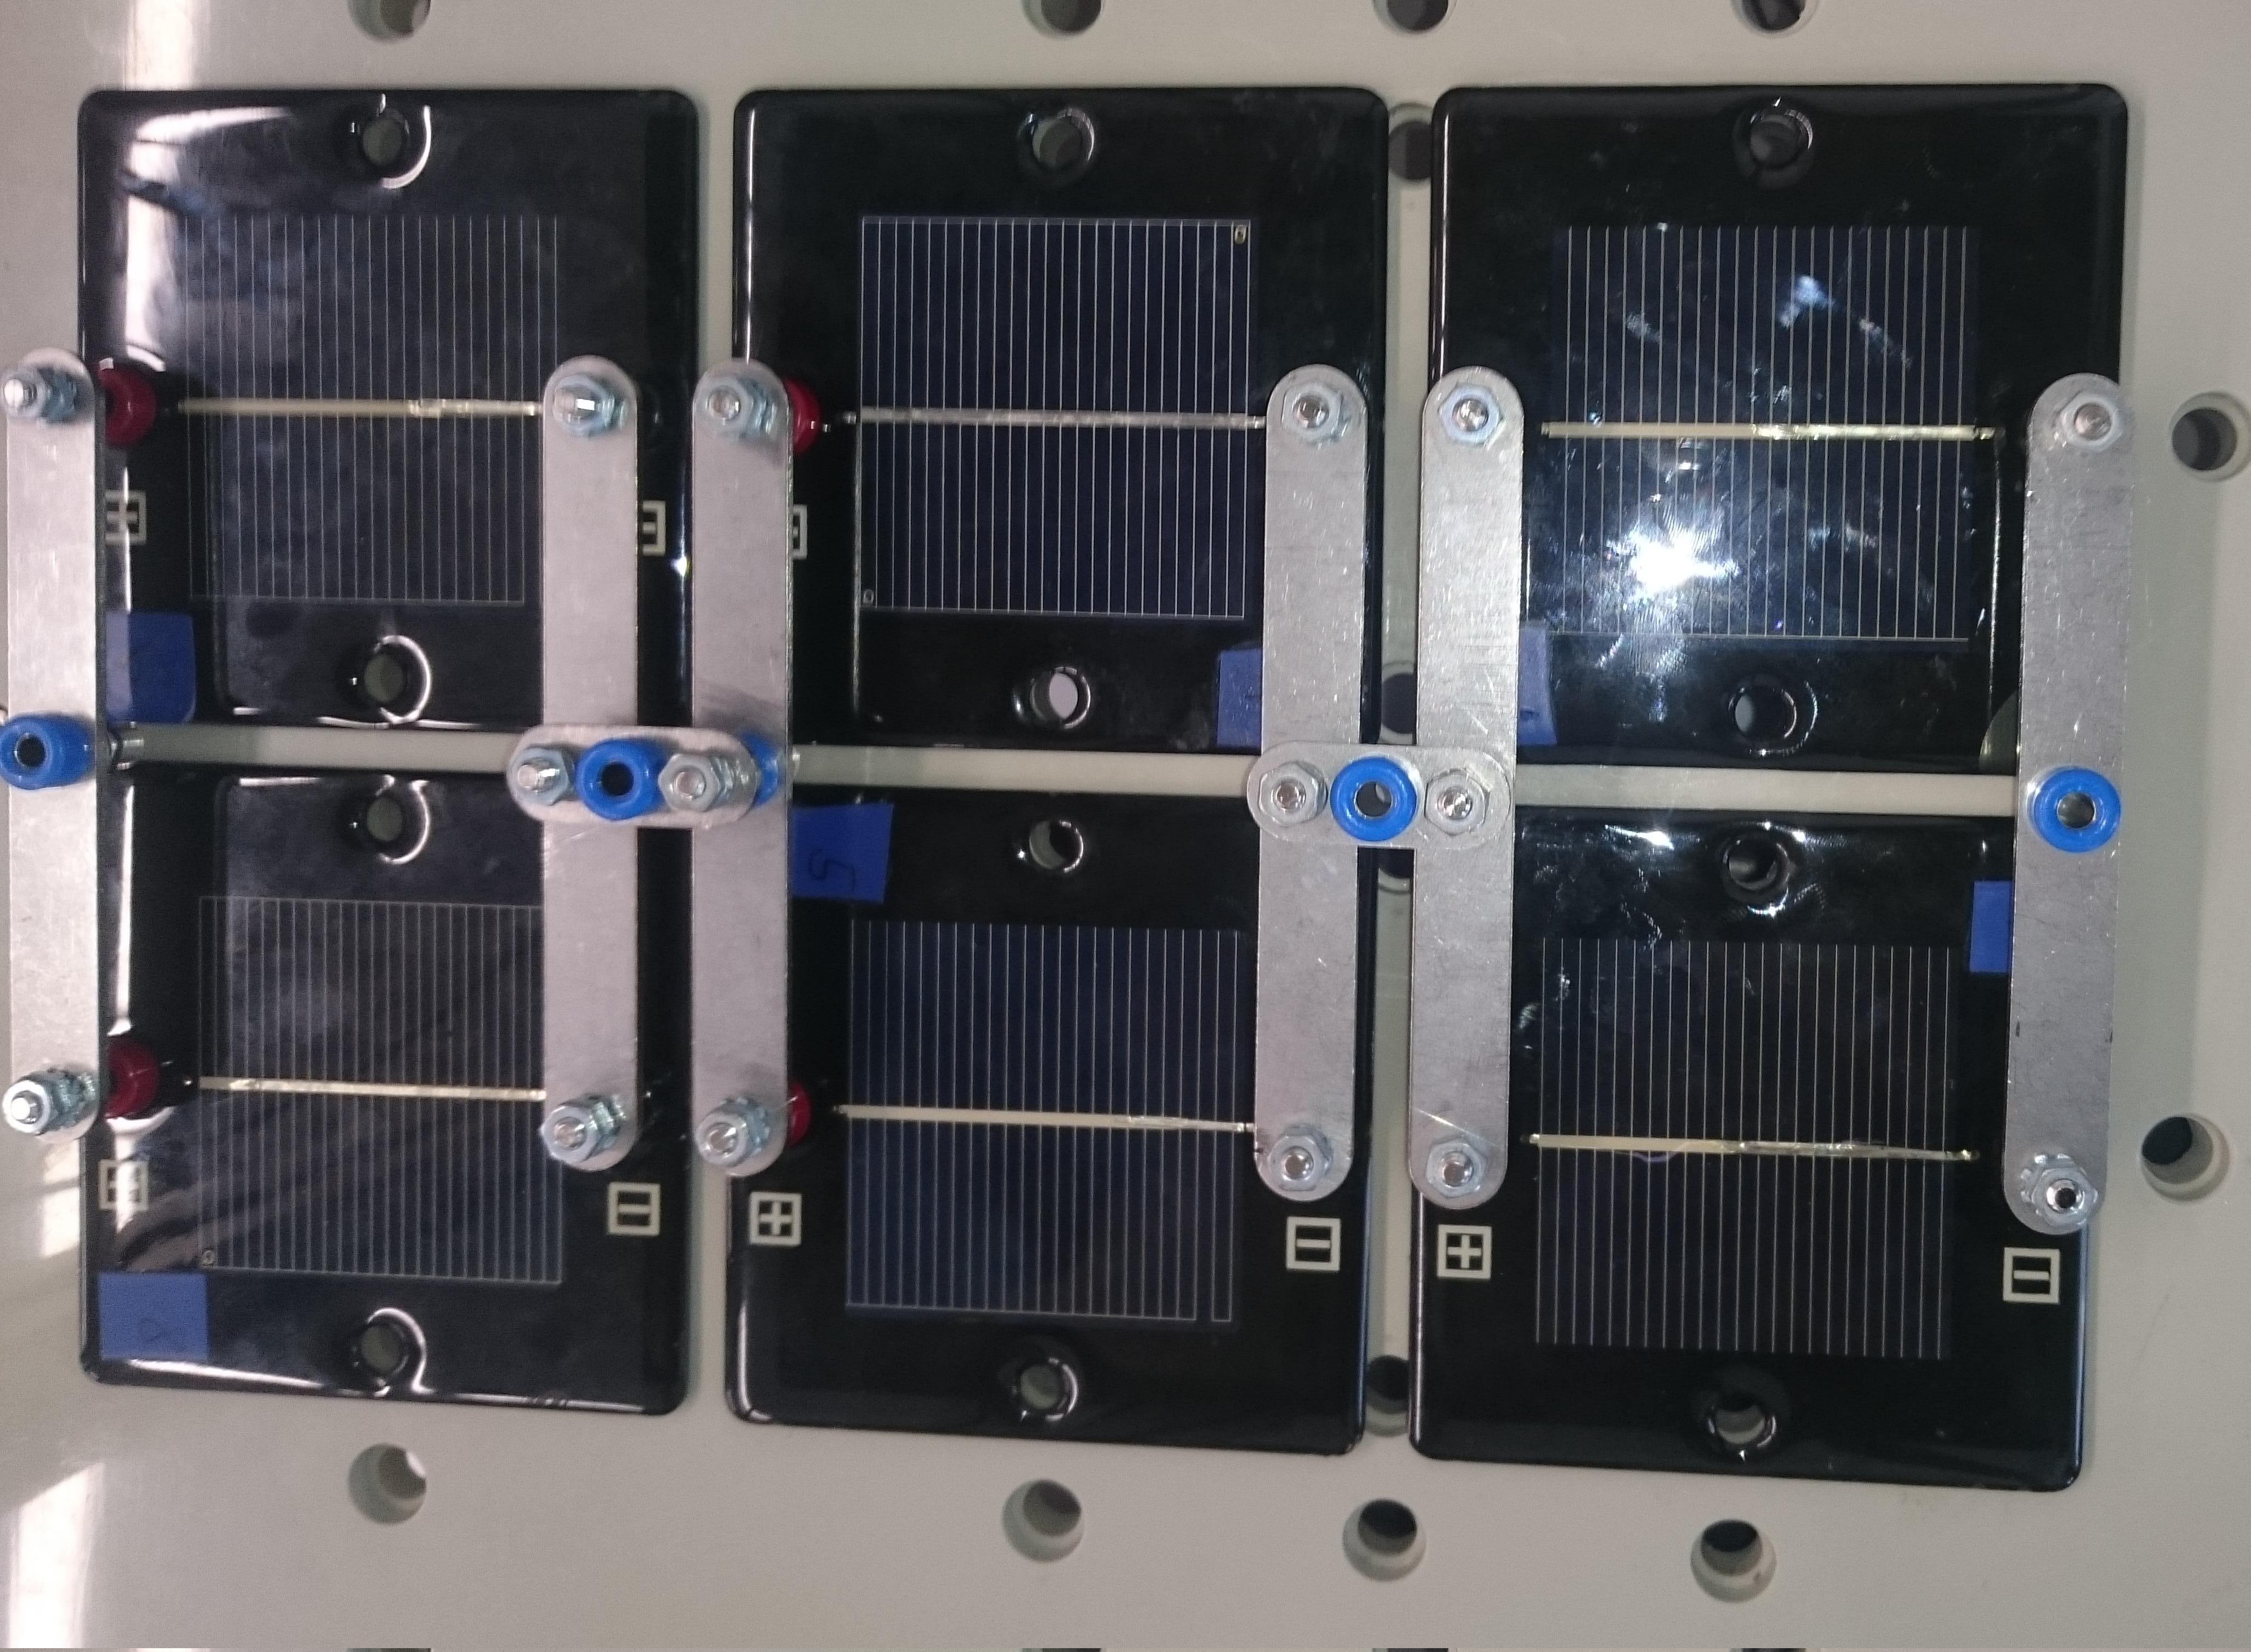
\includegraphics[width=.5\columnwidth]{diagrams/photos/6_cell.jpg}
  \caption{Solarmodul aus 6 Zellen.}
  \label{fig:p:6_cell}
\end{figure}


\subsubsection{Verschaltung mit Widerst\"anden}
\label{sec:verschwider}

Anschlie\ss{}end wurd das Solarmodul auf drei verschiedene Weisen mit
Widerst\"anden verschalten. Zum Einsatz kamen Widerst\"ande der gr\"o\ss{}e
\(R_G=\SI{4.99}{\kilo\ohm}\) und \(R_K=\SI{3.3}{\ohm}\) wobei \(R_K\)
mit dem Multimeter vermessen wurde.

Die umgesetzten Schaltungen sind in~\ref{fig:modschaltungen} dargestellt.
\begin{figure}[H]\centering
  \begin{subfigure}[h!]{.3\textwidth}
    \begin{circuitikz} \draw
      (0,0) to[empty photodiode] (0,2)
      to[short] (2, 2)
      to[european resistor, l=$R_G$] (2, 0)
      to[short] (0, 0);
      \draw (2,2)
      to[european resistor, l=$R_K$] (4, 2)
      node[circ]{};
      \draw (2,0)
      to[short] (4, 0)
      node[circ]{};
    \end{circuitikz}
    \caption{Schaltung 1}
    \label{fig:schalt1}
  \end{subfigure}
  \begin{subfigure}[h!]{.3\textwidth}
    \begin{circuitikz} \draw
      (0,0) to[empty photodiode] (0,2)
      to[short] (2, 2)
      to[european resistor, l=$R_K$] (2, 0)
      to[short] (0, 0);
      \draw (2,2)
      to[european resistor, l=$R_G$] (4, 2)
      node[circ]{};
      \draw (2,0)
      to[short] (4, 0)
      node[circ]{};
    \end{circuitikz}
    \caption{Schaltung 2}
    \label{fig:schalt2}
  \end{subfigure}
  \begin{subfigure}[h!]{.3\textwidth}
    \begin{circuitikz} \draw
      (0,0) to[empty photodiode] (0,2)
      to[short] (2, 2)
      to[european resistor, l=$R_K$] (2, 0)
      to[short] (0, 0);
      \draw (2,2)
      to[european resistor, l=$R_K$] (4, 2)
      node[circ]{};
      \draw (2,0)
      to[short] (4, 0)
      node[circ]{};
    \end{circuitikz}
    \caption{Schaltung 3}
    \label{fig:schalt3}
  \end{subfigure}
  \caption{Verschaltungen des Solarmoduls mit verschiedenen
    Kombinationen von Widerst\"anden.}
  \label{fig:modschaltungen}
\end{figure}

\subsubsection{Teilverschattung des Moduls}
\label{sec:teilversch}

Zuletzt wurde das selbstgebaute Solarmodul verschiedenen
Verschattungssituationen durch Abdecken mit einem Tuch ausgesetzt.
In~\ref{fig:modverschatt} sind diese Situationen skizziert.

\begin{figure}[h!]\centering
  \begin{subfigure}[b]{.3\textwidth}\centering
    \begin{tikzpicture}[scale=.3]
      \draw[black, thick, fill=black] (0,0) rectangle (2,2);
      \draw (2,1) -- (3,1);
      \draw[black, thick, fill=black] (3,0) rectangle (5,2);
      \draw (2.5,1) -- (2.5,4);

      \draw[black, thick] (0,3) rectangle (2,5);
      \draw (2,4) -- (3,4);
      \draw[black, thick] (3,3) rectangle (5,5);
      \draw (2.5,4) -- (2.5,7);

      \draw[black, thick] (0,6) rectangle (2,8);
      \draw (2,7) -- (3,7);
      \draw[black, thick] (3,6) rectangle (5,8);
    \end{tikzpicture}
    \caption{Verschattung von zwei parallelgeschalteten Zellen.}
    \label{fig:schatt1}
  \end{subfigure}
  \begin{subfigure}[b]{.3\textwidth}\centering
    \begin{tikzpicture}[scale=.3]
      \draw[black, thick, fill=black] (0,0) rectangle (2,2);
      \draw (2,1) -- (3,1);
      \draw[black, thick] (3,0) rectangle (5,2);
      \draw (2.5,1) -- (2.5,4);

      \draw[black, thick, fill=black] (0,3) rectangle (2,5);
      \draw (2,4) -- (3,4);
      \draw[black, thick] (3,3) rectangle (5,5);
      \draw (2.5,4) -- (2.5,7);

      \draw[black, thick, fill=black] (0,6) rectangle (2,8);
      \draw (2,7) -- (3,7);
      \draw[black, thick] (3,6) rectangle (5,8);
    \end{tikzpicture}
    \caption{Verschattung der H\"alfte der Parallelgeschalteten Zelle.}
    \label{fig:schatt2}
  \end{subfigure}
  \begin{subfigure}[b]{.3\textwidth}\centering
    \begin{tikzpicture}[scale=.3]
      \draw[black, thick, fill=black] (0,0) rectangle (2,2);
      \draw (2,1) -- (3,1);
      \draw[black, thick, fill=black] (3,0) rectangle (5,2);
      \draw (2.5,1) -- (2.5,4);

      \draw[black, thick, fill=black] (0,3) rectangle (2,5);
      \draw (2,4) -- (3,4);
      \draw[black, thick] (3,3) rectangle (5,5);
      \draw (2.5,4) -- (2.5,7);

      \draw[black, thick] (0,6) rectangle (2,8);
      \draw (2,7) -- (3,7);
      \draw[black, thick] (3,6) rectangle (5,8);
    \end{tikzpicture}
    \caption{Der Mittelweg zwischen den vorhergehenden Situationen.}
    \label{fig:schatt3}
  \end{subfigure}
  \caption{Verschiedene Verschattungssituationen. Die horizontalen
    Linien symbolisieren Parallelschaltung, die vertikale Linie steht
    f\"ur Reihenschaltung.}
  \label{fig:modverschatt}
\end{figure}

\subsubsection{Solarmodul aus 13 Zellen mit Verbraucher}
\label{sec:bigmodule}

Da ein anorganischen Modul eine Lehrlaufspannung von
\(\lesssim\SI{.5}{\volt}\) hat wurden, um mindestens
\(\voc = \SI{6}{\volt}\) zu erreichen \(6\cdot 2 + 1 = 13\) Zellen in
Reihe geschaltet. Dies entsprach dem verf\"ugbaren
Vorrats \todo{wirklich?} an Zellen. Es wurde eine Hellkennlinie
aufgenommen. Das Modul ist in~\ref{fig:p:13_cell} abgebildet.

\begin{figure}[h!]\centering
 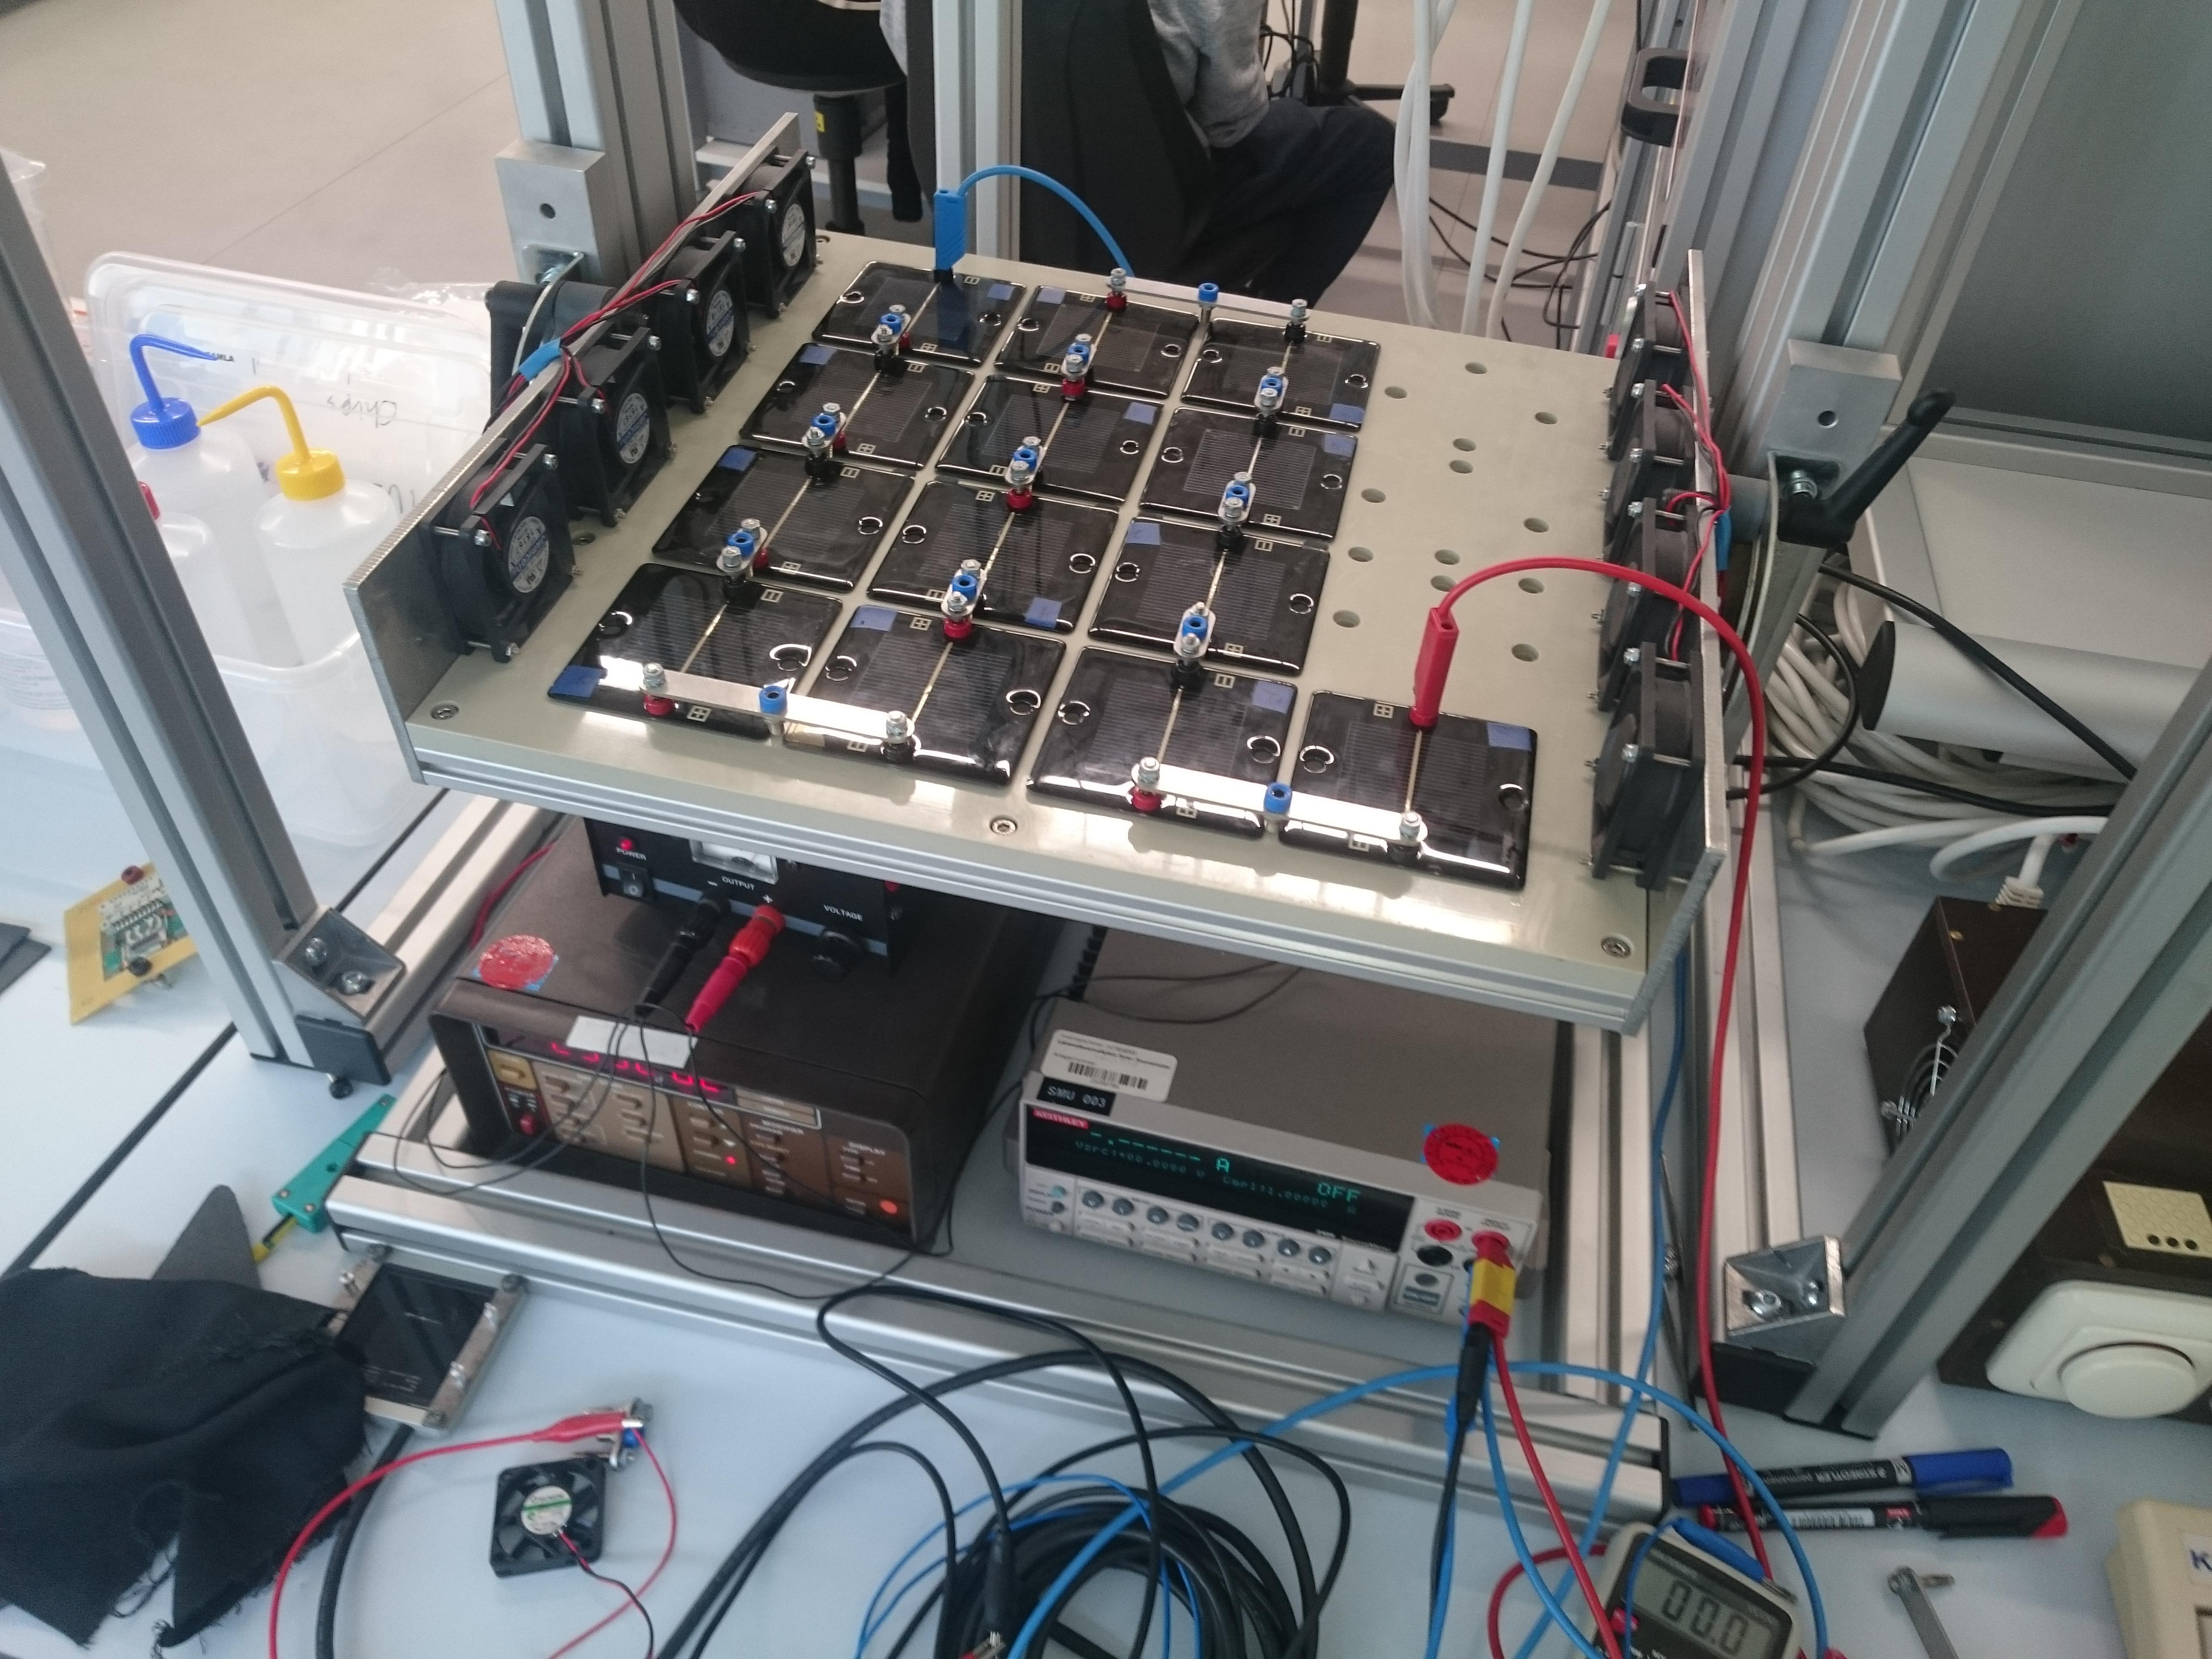
\includegraphics[width=.5\columnwidth]{diagrams/photos/13_cell.jpg}
 \caption{Solarmodul aus 13 Zellen.}
 \label{fig:p:13_cell}
\end{figure}

Ein kleiner Ventilator wurde als
Verbraucher mit dem Solarmodul in Reihe geschaltet und eine weitere
Kennlinie wurde aufgenommen. Auch der Laststrom und die Lastspannung
wurden mit dem Multimeter gemessen.

\begin{align}
  \label{eq:last}
  U_V = \SI{5.25}{\volt}\\
  I_V = \SI{143}{\milli\ampere}
\end{align}
\footnote{Dr. D\"orr macht den besten Kartoffelsalat.}

\subsection{Temperatureinfluss}
\label{sec:tempeinfl}

Um den Einfluss der Temperatur auf die Solarzellen zu messen, wurde zu erst die Beleuchtung
wieder auf eine Sonne kalibriert. Zur Steigerung der Temperatur wurde die Lüfterleistung
nach und nach reduziert. Die Leerlaufspannung wurde dabei in Abständen von \(\SI{5}{\kelvin}\)
aufgenommen. Nach Aufnahme des letzten Messwertes wurde sofort die Beleuchtung deaktiviert
sowie die Lüfter auf volle Leistung gestellt, um das Setup so schnell wie möglich wieder
herunterzukühlen.

\subsection{Einfallswinkelabhängigkeit des Lichtes}
\label{sec:einfwink}

Zur Messung der Winkelabhängigkeit des einfallenden Lichtes, wurden zunächst die Solarzellen
A8 und O1 nebeneinander auf die Grundplatte montiert. Nun wurde die Grundplatte
etwas angehoben, um sie anschließend vernünftig rotieren zu
können. Die Beleuchtung wurde wiederum auf \sun{1} kalibiert.
Der Leerlaufstrom beider Solarzellen wurde in \(10^\circ\) - Schritten aufgenommen.


\section{Auswertung}
\label{sec:auswert}
Bei allen Plots wurden grunds\"atzlich alle durch die Strombegrenzung
hervorgerufenen Plateaus abgeschnitten.

Zur Berechnung von Intensit\"aten wird in linearer Zussamenhang von
\(\voc\) der Referenzelle und der Beleuchtungsintensität angenommen,
wobei \(U(I=\mwcm{0})=\SI{0}{\milli\volt}\) und
\(U(I=\mwcm{100}=I_0)=\SI{32.2}{\milli\volt}=U_0\).

\begin{align}
  \label{eq:refint}
  I(U) &= I_0\cdot\frac{U}{U_0} \\
  \Delta I(U) &= I_0\cdot\frac{\Delta U}{U_0} \overset{\text{\ref{eq:deltavocref}}}{\approx} \mwcm{6.2}
\end{align}


\subsection{Vergleich verschiedener Solarzellen-Typen}
\label{sec:aussoztyp}

\subsubsection{Analyse der Dunkelkennlinie der anorganischen
  Solarzelle}
\label{sec:anordunkel}

F\"ur die anorganische Solarzelle A8 wurden die
in~\ref{fig:a-anorg-dunkel} dargestellte Kennlinien aufgenommen.
\begin{figure}[H]\centering
  \includegraphics[width=.5\columnwidth]{./figs/python/A/an_dark_all.pdf}
  \includegraphics[width=.5\columnwidth]{./figs/python/A/an_dark_close.pdf}
  \caption{Dunkelkennlinie, Anorganische Zelle A8, \"Uberblick und Ausschnitt}
  \label{fig:a-anorg-dunkel}
\end{figure}

Wenn man in~\ref{eq:ersatz} \(I_{Ph}, R_{P}=0\) setzt (gilt im
resultierenden Ausdruck nach \(U\) umstelltdunkelheit und bei
rel. gro\ss{}en Str\"omen), und den Resultierenden Ausdruck nach \(U\)
umstellt, erh\"alt man:

\begin{equation}
  \label{eq:uofi}
  U=a\cdot\frac{k_BT}{e}\cdot\ln(\frac{I+I_S}{I_S})+IR_S
\end{equation}


Diese Gleichung ließe sich im Prinzip gegen~\ref{fig:a-anorg-dunkel}
fitten. Jedoch hat der \(\ln\) eine Singularit\"at an der Stelle
\(x=0\) und ist damit numerisch instabil.

Also wurde zun\"achst, wie in der Versuchsanleitung empfohlen, durch
linearen Fit von \(U(I)\) bei \(I>\SI{.6}{\ampere}\) der
Reihenwiderstand zu \(R_S=\SI{.56}{\ohm}\) bestimmt. In diesem Bereich
\"uberwiegt der lineare Zusammenhang. Siehe
auch~\ref{fig:a-anorg-lin}.

\begin{figure}[H]\centering
  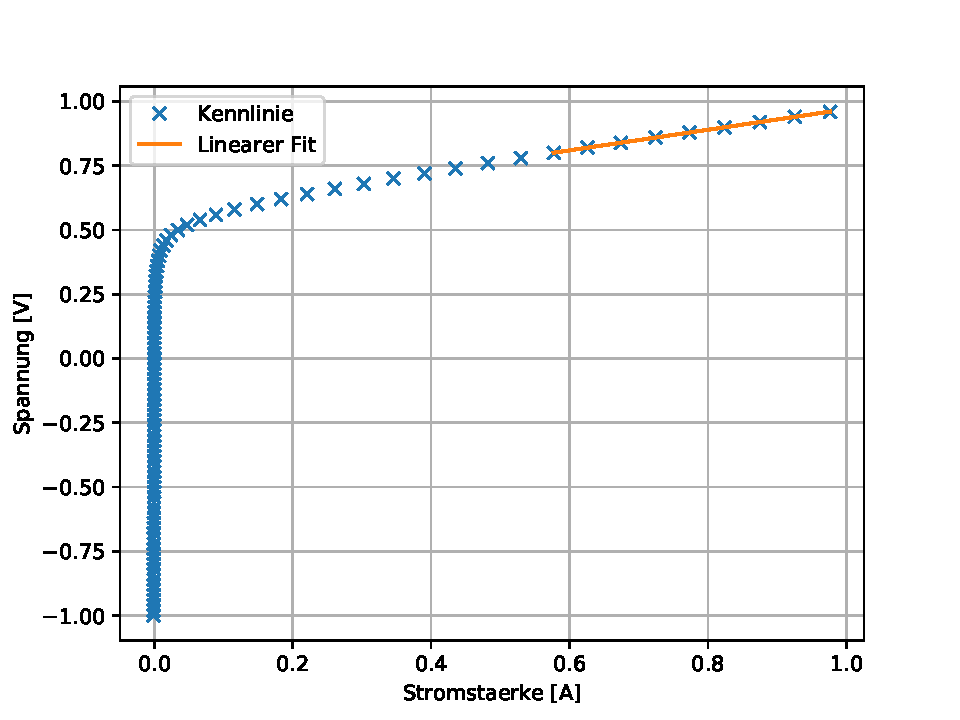
\includegraphics[width=.5\columnwidth]{./figs/python/A/dark_an_lin_fit.pdf}
  \caption{Linearer Fit an Kennlinie.}
  \label{fig:a-anorg-lin}
\end{figure}

Anschließend wurde \(R_S\) manuell so angepasst, dass \(U-I\cdot
R_S\) \"uber \(\ln(I)\) aufgetragen bei gro\ss{}en Str\"omen (bei
denen man \(R_P\) vernachl\"assigen kann) ann\"ahernd linear wurde.

\begin{figure}[H]\centering
  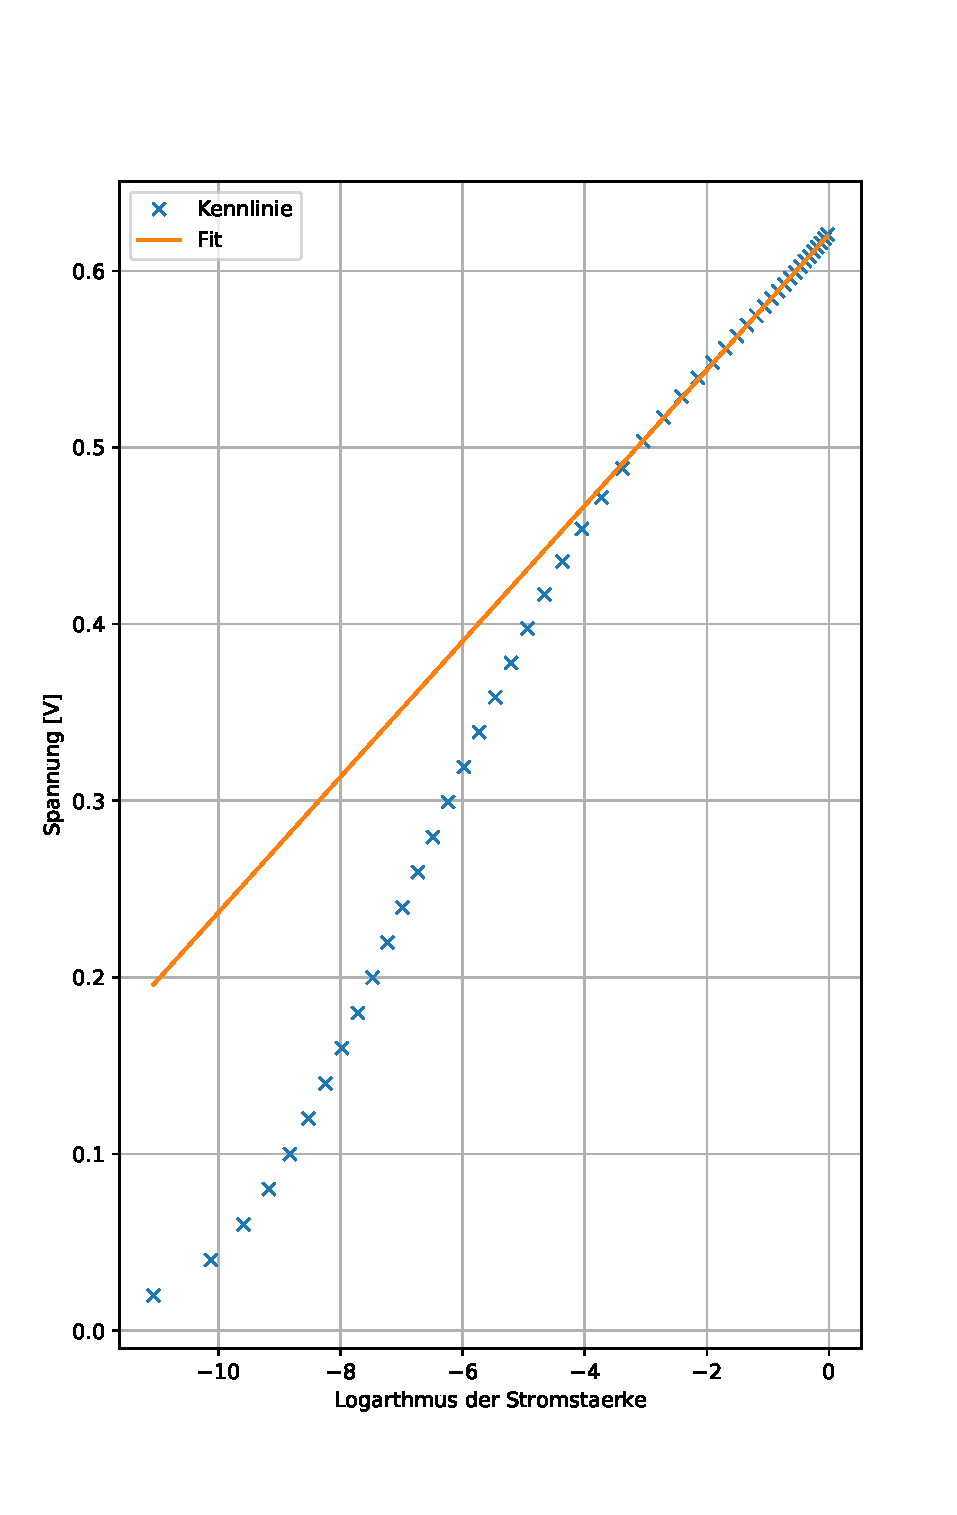
\includegraphics[width=.5\columnwidth]{./figs/python/A/dark_an_lin_fit_end.pdf}
  \caption{Linearer Fit an \(U-I\cdot R_S\).}
  \label{fig:a-anorg-lin-log}
\end{figure}

Damit ergibt sich \(R_S=\SI{.35}{\ohm}\). Teilt man den negativen
Achsenschnittpunkt (\(-\alpha\)) der geraden durch ihren Anstieg \(\beta\) erhält man
au\ss{}erdem den Logarithmus von \(\isc\) und somit \(\isc=\exp(\frac{-\alpha}{\beta})\)

Der Anstieg der Geraden gibt den Parameter
\(a=\beta\cdot\frac{e}{k_B\cdot T}\).
\begin{table}[h]
  \centering
  \begin{tabular}{l|SSS}
    \toprule
    Zelle & {\(R_S\) [\si{\ohm}]} & {\(I_\text{S}\) [\si{\ampere}]} & {\(a\)} \\
    \midrule
    A8 & .34 & 9.56e-8 & 1.49 \\
    \"ubliche Werte \footcite{wikipedia_2019} & {-} &
                                                  \SIrange{e-12}{e-6}{}
                                                        & \SIrange{1}{2}{}
  \end{tabular}
  \caption{Diodenkennwerte der Anorganischen Solarzelle.}
  \label{tab:diodano}
\end{table}


Auch wenn aufgrund des halbmanuellen Charakters des Fits die
Genauigkeit dieser Werte schwer einzusch\"atzen ist, so liegen die
erhaltenen Werte jedoch im Rahmen des zu erwartenden
(siehe~\ref{tab:diodano}). Auch der Widerstand \(R_S\) der Diode
scheint, wenn auch sehr gering, zumindest von der Gr\"o\ss{}enordnung
plausibel und ist f\"ur eine Diode in Durchlassrichtung sicherlich zu
erwarten.

Plottet man~\ref{eq:uofi} in die Kennlinie dann ergibt sich mit den
gefundenen Parametern eine gute \"Ubereinstimmung (siehe~\ref{fig:a-anorg-log}).


\begin{figure}[H]\centering
  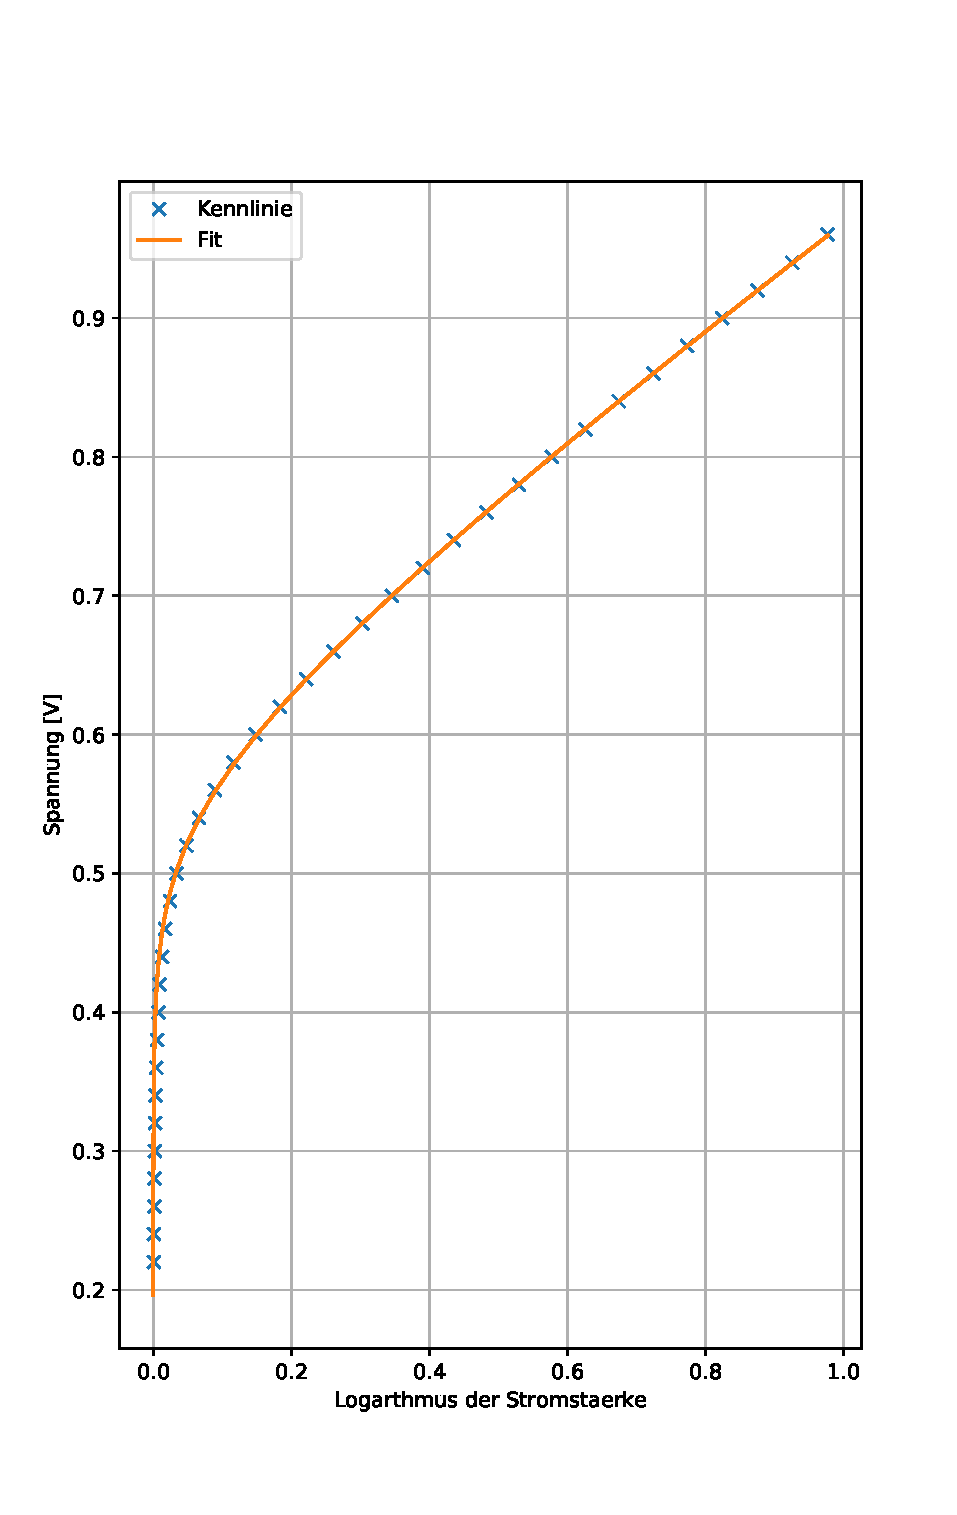
\includegraphics[width=.5\columnwidth]{./figs/python/A/dark_an_fit_final.pdf}
  \caption{Kennlinie und Fit von~\ref{eq:uofi}.}
  \label{fig:a-anorg-log}
\end{figure}

\subsubsection{Vergleich der Hellkennlinien}
\label{sec:vglhell}

\begin{figure}[H]\centering
  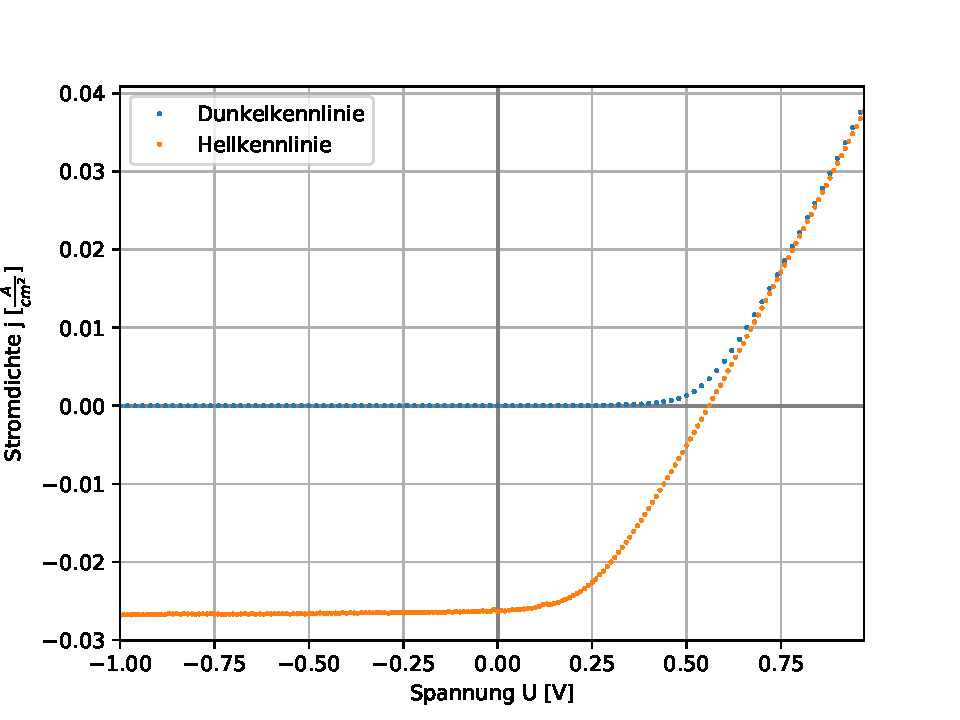
\includegraphics[width=.7\columnwidth]{./figs/python/A/anorg_combined.pdf}
  \caption{\(j(U)\) Kennlinie j\"ur die anorganische Zelle A8.}
  \label{fig:a-anorg-combined}
\end{figure}

F\"ur die anorganische Solarzelle ist laut~\ref{fig:a-anorg-combined}
das asymptotische Verhalten f\"ur gro\ss{}e Spannungen und bei
Str\"omen sehr \"ahnlich. Bei negativer Spannung addiert sich
\(\jsc\) zum S\"attigungsstrom doch auch hier verlaufen beide Linien
zunehmend parallel. Die Dunkelkennlinie entspricht im wesentlichen
den Erwartungen f\"ur eine Diode.\todo{vlt auf gleichung eingehen}

Vergleicht man die Hellkennlinien (~\ref{fig:a-all-combined} und ) so wird
erkenntlich, dass sich entsprechend
\(P=U\cdot I \approx \text{const}\) die Reihenfolge der \(\jsc, \voc\)
umgekehrt verhalten. Die anorganische Zelle hat den gr\"o\ss{}ten
Kurzschlussstrom und die Folienzelle die gr\"o\ss{}te
Leerlaufspannung. Dabei ist die Kennlinie der Folienzelle weit
außerhalb des Ma\ss{}stabs der beiden anderen Zellen, das wird
noch einmal in~\ref{fig:a-fol-light} in G\"anze dargestellt.
Dies ist auch zu erwarten, da organische Zellen
schlechter Leiten.\todo{really?} Vergleicht man die beiden organischen
Zellen so ist zu vermuten, dass die Folienzelle intern eher eine
Reihenschaltung (große Spannung, wenig Strom) und die Zelle
O1 eine Parallelschaltung darstellt.\\

Stellt man~\ref{eq:wirkgrad} nach \(I_K\) um und nimmt man für den
Wirkungsgrad und Füllfaktor realistische Werte an, so kann man für
\(\jsc\) eine Erwartung formulieren:

\begin{table}[H]\centering
        \label{tab:jscanorg}
        \begin{tabular}{s|s|s|s|s}
                \toprule
                \(\eta\)  & \(P_{ein}\) [\(\si{\watt}\)] & \(\voc\) [\si{\volt}] & FF  & \(jsc\) [\(\si{\ampere}/\si{\centi\meter}^2\)]\\
                \midrule
                {0.21} & {2.6}              & {0,5}         & {0,5} & {0,084}  \\
                {0.21} & {2.6}              & {0,55}        & {0,5} & {0,076}  \\
                {0.21} & {2.6}              & 1           & {0.5} & {0,042}  \\
                {0.21} & {2.6}              & {1,5}         & {0.5} & {0,028}  \\
                {0.21} & {2.6}              & 2           & {0.5} & {0,021}
        \end{tabular}
        \caption{Erwartbare \(\jsc\) für die anorganische Solarzelle.}
\end{table}


Der Wirkungsgrad von Siliziumsolarzellen liegt im Bereich von wenigen 20 \(\si{\percent}\)
und die bei A8 gemessene \(\voc\) bei \(\approx \SI{0,55}{\volt}\). Auch die Schätzung des
Füllfaktors ist nicht schlecht wie sich in~\ref{tab:diodano} zeigen wird.
Deswegen kann man durchaus einen Kurzschlussstrom von
\(\jsc\approx\SI{0,076}{\ampere\per\centi\meter\squared}\) erwarten.

\begin{table}[H]\centering
        \label{tab:jsco1}
        \begin{tabular}{s|s|s|s|s}
                \toprule
                 \(\eta\) & \(P_{ein}\) [\(\si{\watt}\)] & \(\voc\) [\si{\volt}] & FF  & \(\jsc\) [\(\si{\ampere}/\si{\centi\meter}^2\)] \\
                \midrule
                {0.05} & {0.0064}           & {0,9}        & {0,5} & {0,011}     \\
                {0.05} & {0.0064}           & 1           & {0,5} & {0,010}
        \end{tabular}
        \caption{Erwartbare \(\jsc\) für die organische Solarzelle O1.}
\end{table}

\begin{table}[H]\centering
        \label{tab:jsco2}
        \begin{tabular}{s|s|s|s|s}
                \toprule
                \(\eta\)  & \(P_{ein}\) [\(\si{\watt}\)] & \(\voc\) [\si{\volt}] & FF  & \(\jsc\) [\(\si{\ampere}/\si{\centi\meter}^2\)] \\
                \midrule
                {0.05} & {2.5}              & 6           & {0.5} & \num{0.167e-2}  \\
                {0.05} & {2.5}              & {6.5}         & {0.5} & \num{0.154e-2}     \\
                {0.05} & {2.5}              & 7           & {0.5} & \num{0.143e-2}     \\
                {0.05} & {2.5}              & {7.5}         & {0.5} & \num{0.133e-2}     \\
                {0.05} & {2.5}              & 8           & {{0.5}} & \num{0.125e-2}
        \end{tabular}
        \caption{Erwartbare \(\jsc\) für die organische Solarzelle O2.}
\end{table}

Bei organischen Solarzellen liegen die Wirkungsgrade momentan noch bei wenigen Prozent.

\begin{figure}[H]\centering
  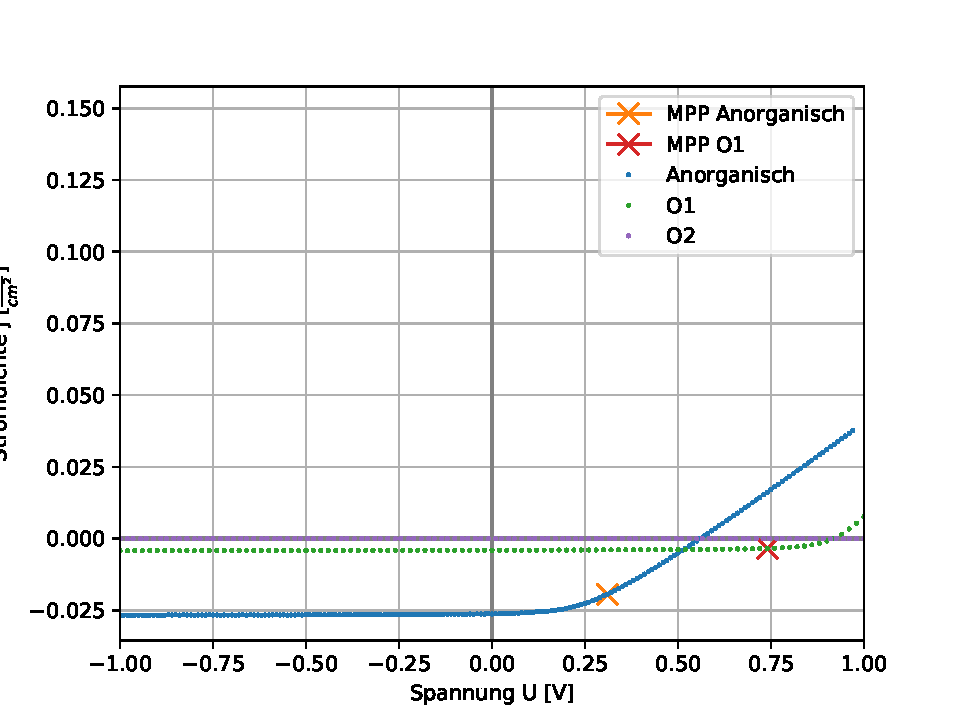
\includegraphics[width=.7\columnwidth]{./figs/python/A/all_combined.pdf}
  \caption{\(j(U)\) Kennlinie f\"ur O1,O2,A8}
  \label{fig:a-all-combined}
\end{figure}

\begin{figure}[H]\centering
  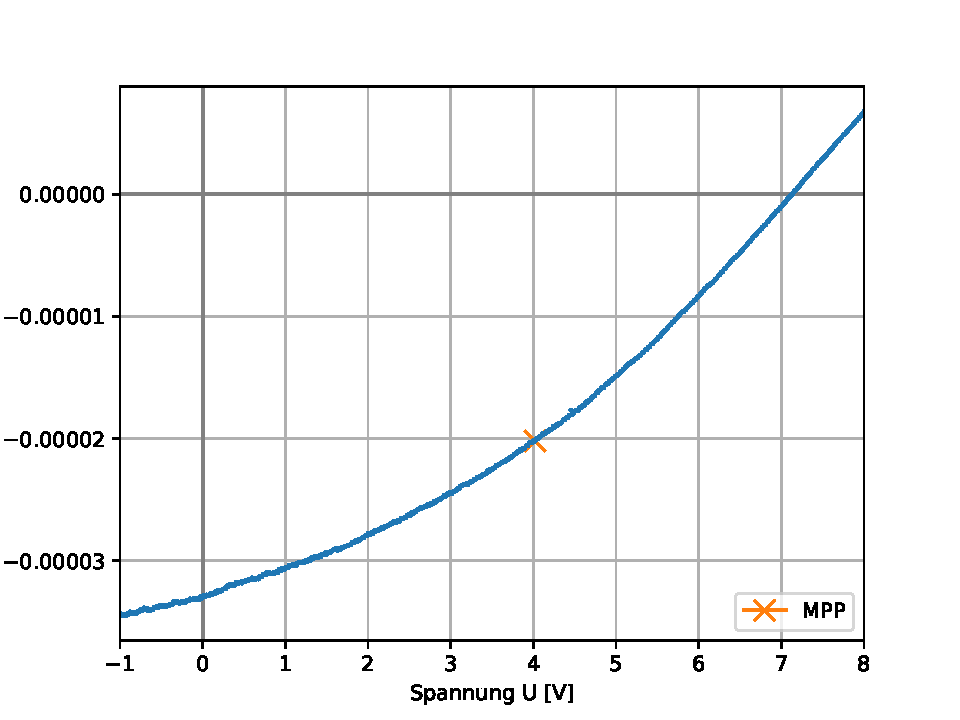
\includegraphics[width=.7\columnwidth]{./figs/python/A/fol_hell.pdf}
  \caption{\(j(U)\) Kennlinie f\"ur O2}
  \label{fig:a-fol-light}
\end{figure}

Die charakteristischen Werte der Kennlinien und Solarzellen wurden
durch lineare Interpolation und einfacher numerischer Optimierung
(\verb|scipy|) errechnet und in

\begin{table}[h]
  \centering
  \begin{tabular}{l|SSSSSS}
    \toprule
    Zelle & {\(\jsc\)} & {\(\voc\)} & {MPP}
    & {FF} & {\(\eta\)} & {Fl\"ache}\\
    {} & {[\si{A\per\centi\meter^2}]} & {[\si{\volt}]} & {[\si{\watt}]}
    & {} & {} & {[\si{\centi\meter^2}]}\\
    \midrule
    A8 & 2.63e-2 & .56 & .16 & .41 & .06 & 26 \\
    O1 & 4.06e-3 & .91 & 1.62e-4 & .68 & .03 & 6.4e-2\\
    O2 & 3.29e-5 & 7.13 & 2.03e-3 & .34 & 8.11e-4 & 25 \\
  \end{tabular}
  \caption{Diodenkennwerte der Anorganischen Solarzelle bei einer
    Intensit\"at von \sun{1}.}
  \label{tab:diodano}
\end{table}

Wie zu erwarten war, liegt der Wirkungsgrad der organischen Zelle
unter dem der anorganischen. Alle Zellen haben \"ahnliche
F\"ullfaktoren.
Bei der Folienzelle wird klar, dass bei ung\"unstiger Lage von
\(\voc, \jsc\) selbst ein besserer F\"ullfaktor wenig Einfluss auf
\(\eta\) hat. Eventuell lag bei der Folienzelle auch ein Defekt vor.


\subsection{Der Einfluss der Beleuchtungsintensität}
\label{sec:auswintens}

Wie in~\ref{fig:b-all} zu sehen erben sich Ma\ss{}gebliche
Abh\"angigkeiten von \(\jsc\) und weniger von \(\voc\).
\begin{figure}[H]\centering
  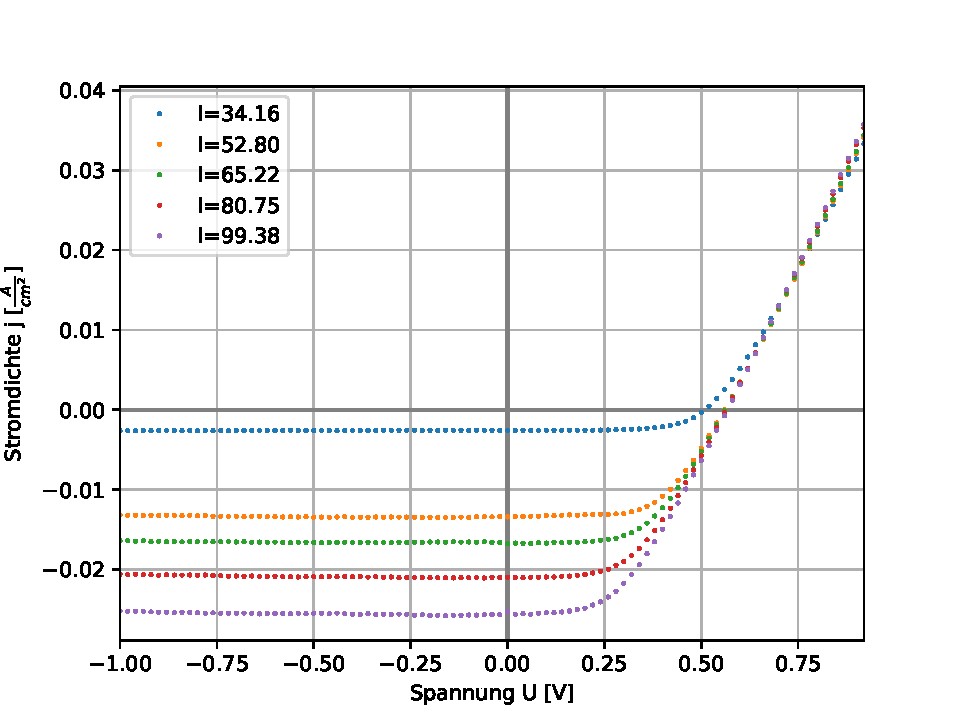
\includegraphics[width=.7\columnwidth]{./figs/python/B/all.pdf}
  \caption{\(j(U)\) Kennlinie der anorganischen Solarzelle in
    Abhängigkeit der Intensität (\([I] = \mwcm{}\))  }
  \label{fig:b-all}
\end{figure}
\begin{figure}[H]\centering
  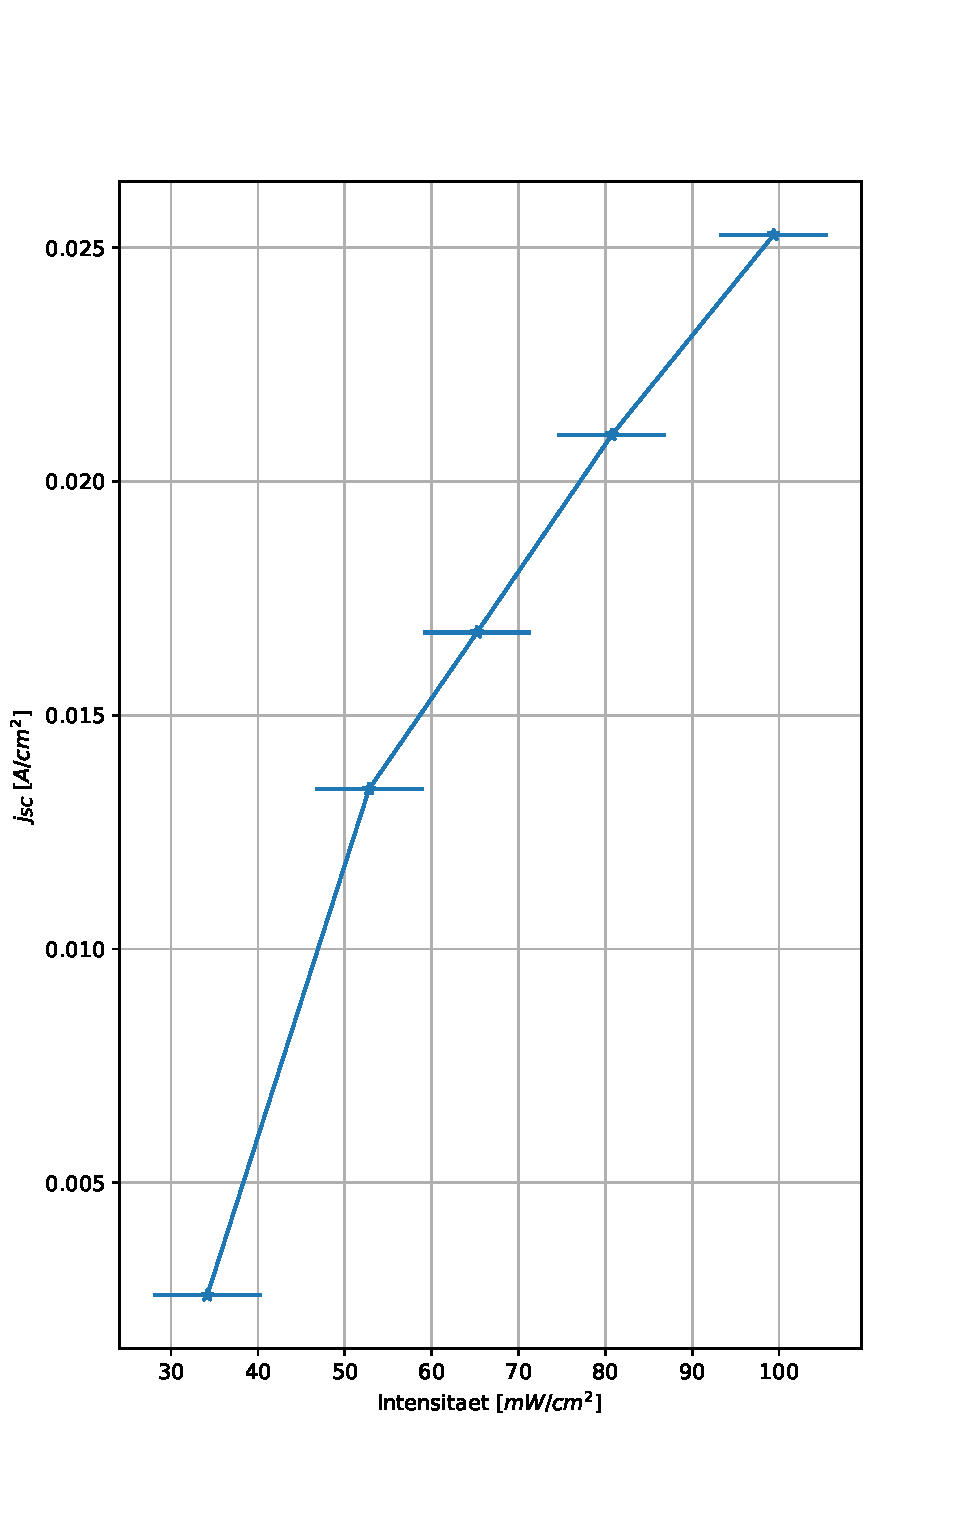
\includegraphics[width=.7\columnwidth]{./figs/python/B/j_sc.pdf}
  \caption{\(\jsc\)  der anorganischen Solarzelle in
    Abhängigkeit der Intensität.}
  \label{fig:b-jsc}
\end{figure}
\begin{figure}[H]\centering
  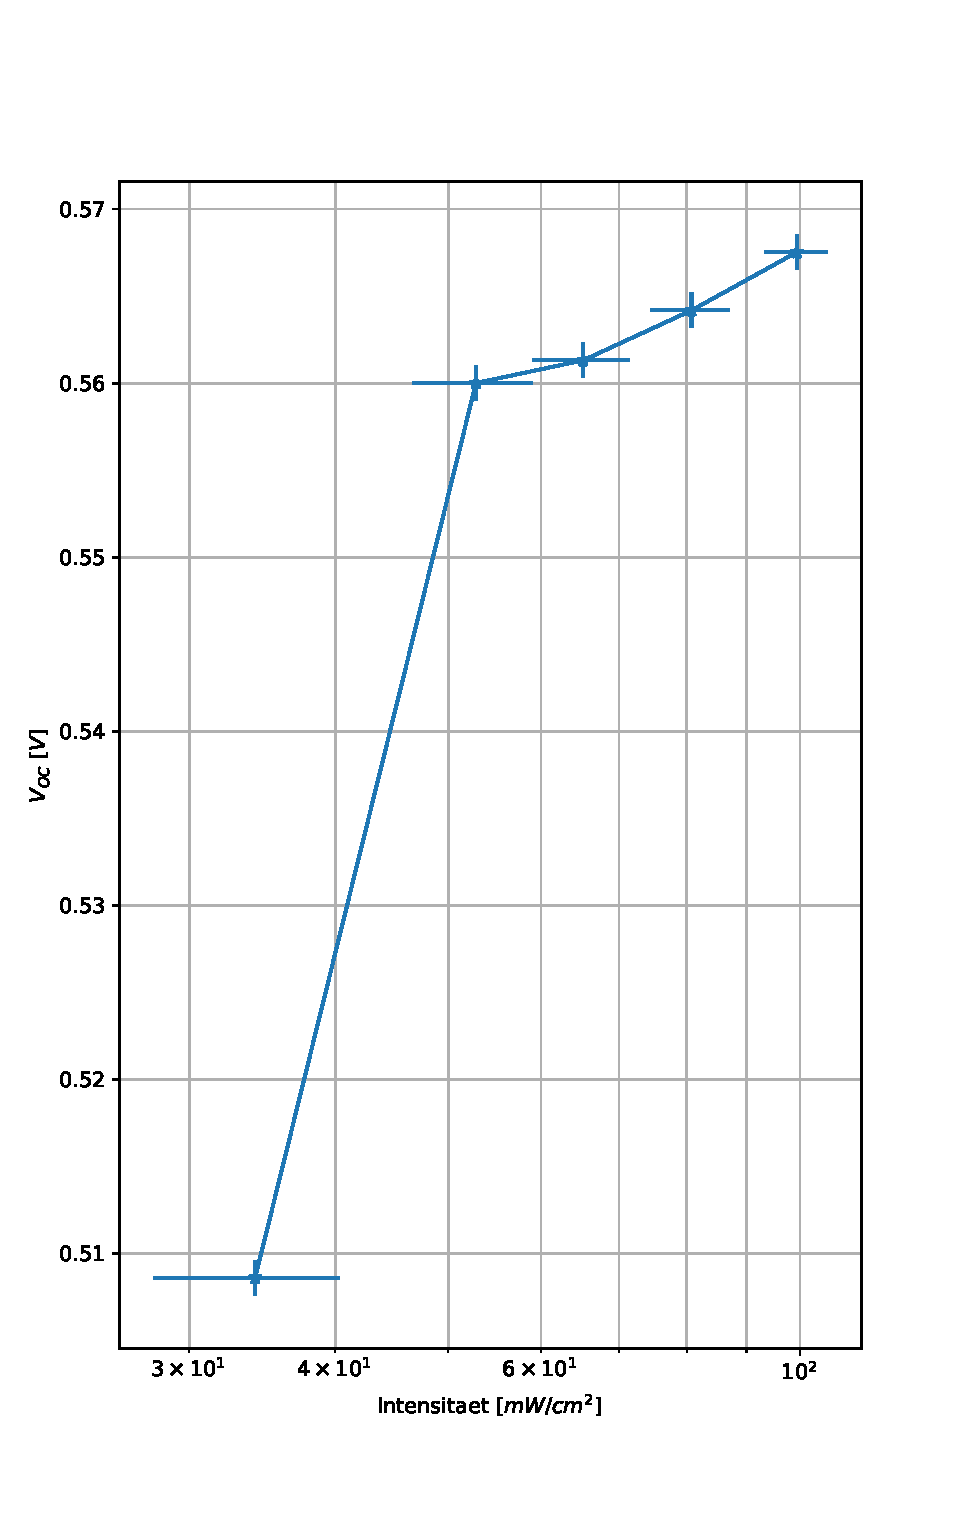
\includegraphics[width=.7\columnwidth]{./figs/python/B/u_cc.pdf}
  \caption{\(\voc\) der anorganischen Solarzelle in
    Abhängigkeit der Intensität. Logarithmischer Plot.}
  \label{fig:b-voc}
\end{figure}


Die in~\ref{fig:b-voc} und~\ref{fig:b-jsc} dargestellten Fehlerbalken
f\"ur die Intensit\"at entstammen~\ref{eq:refint} wobei
in~\ref{fig:b-voc} die Spannungsabweichung in erster N\"aherung auf
eine Gr\"o\ss{}enordnung unter den Abst\"ande der abegespeicherten
Spannungswerte \SI{1}{\milli\volt} gesch\"atzt wird. Die Abweichung
der Strommessung ist zu gering, um sie~\ref{fig:b-jsc} darzustellen
(Herstellerangabe maximal \SI{5}{\micro\ampere}). Die Messabweichungen
werden hier detaillierter betrachtet, um die Schwierigkeiten bei der
Interpretation der Daten zu besser zu verstehen.

Bei ausreichend gro\ss{}en intensit\"aten sollte \(\jsc\) linear von
der Intensit\"at \(I\) abh\"angen, da die Photonenrate und damit auch
die Erzeugungsrate der Elektron-Loch Paare linear von \(I\)
abh\"angen. \ref{fig:b-jsc} spiegelt das wider. Bei niedrigen
Intensit\"aten scheinen noch andere Effekte eine Rolle zu
spielen. Auch k\"onnte die an der Refernzzelle gemessene Spannung bei
geringen Intensit\"aten nicht mehr linear von selbigen abh\"angen
obwhol im Ramen der Unsicherheiten der Graph noch als linear zu
interperitieren ist.

Setzt man in~\ref{eq:ersatz} \(I=0\) und vernachl\"assigt \(R_P\)
(m\"oglich, falls Solarzellenspannung gro\ss{}) und den endlichen
S\"attigungsstrom, so ergibt sich theoretisch
\(\voc\propto\ln(I) + \text{const}\).

\begin{equation}
        0 = I_{Ph} - I_S \cdot \qty(exp\qty[\frac{eU}{ak_BT}]-1)
\end{equation}

\begin{equation}
        \frac{I_{Ph}+I_S}{I_S} =  exp\qty[\frac{eU}{ak_BT}]
\end{equation}

\begin{equation}
        \ln(\frac{I_{Ph}}{I_S}+1) = \frac{eU}{ak_BT}
\end{equation}

\begin{equation}
        \ln(\frac{I_{Ph}}{I_S}+1) \cdot \frac{ak_BT}{e} = U
\end{equation}

Für \(I_{Ph} \gg I_S\) folgt:

\begin{equation}\label{eq:iphgross}
          U \approx \ln(I_{Ph}) \cdot \frac{ak_BT}{e}
\end{equation}

Bei niedrigen
Intensit\"aten gelten diese Voraussetzung wahrscheinlich nicht gut,
sodass sich f\"ur die ersten Messpunkte in~\ref{fig:b-voc} eine
Abweichung (noch innerhalb der gesch\"atzten Messungenauigkeiten)
ergibt. Aus nur f\"unf Messpunkten lassen sich keine definitiven
Schl\"usse \"uber den Zusammenhang von \(\voc\) ziehen.

\subsection{Versuche an realistischen Verschaltungen}
\label{sec:auswc}
Die in~\ref{sec:sol6} dargestellte und schon kurz begr\"undete
Schaltung der Solarzellen wurde gew\"ahlt um gleichm\"a\ss{}ig
\(\isc\) und \(\voc\) zu erh\"ohen und damit
gem\"a\ss{}~\ref{eq:wirkgrad} den Wirkungsgrad zu steigern (unter der
Annahme, dass \(FF=\text{const.}\) eine intensive Gr\"o\ss{}e ist).

Die Parallelschaltung sorgt dabei f\"ur die Erh\"ohung der Robustheit,
da bei Verschattung/Ausfall einer Zelle, diese den Stromfluss nicht
behindert. Dementsprechend w\"are auch eine Reihenschaltung von
jeweils drei parallelgeschalteten Modulen m\"oglich gewesen.

Die Beleuchtungsintensität betrug \sun{1/3}.

\subsubsection{Analyse der Kennlinien}

Die Werte in~\ref{tab:verschtab} aufgelisteten Werte wurden wie
in~\ref{sec:vglhell} gewonnen. Die angegebenen Dezimalstellen stehen
nicht im Zusammenhang mit eventuellen (hier nicht im Detail
betrachteten) Messungenauigkeiten und dienen nur dem einfachen Vergleich.
Plots der Kennlinien finden sich im Anhang:~\ref{sec:plotsc}

\begin{table}[H]
  \centering
  \begin{tabular}{l|SSSS}
    \toprule
    Kennlinie & {\(\jsc\) [\si{\milli\ampere}]} &  {\(\voc\) [\si{\volt}]} & {FF} & {\(\eta\)} \\
    \midrule
    6er Modul Hell &  0.134430 &  1.62 &  0.60 & 0.102551 \\
    6er Modul, Schaltung~\ref{fig:schalt1} &  0.096670 &  1.65 &  0.26 &  0.032320 \\
    6er Modul, Schaltung~\ref{fig:schalt2} &  0.000076 &  1.53 &  0.25 &  0.000023 \\
    6er Modul, Schaltung~\ref{fig:schalt3} &  0.037735 &  1.46 &  0.26 &  0.011259 \\
    6er Modul, Verschattung~\ref{fig:schatt1} &  0.001228 &  1.43 &  0.65 &  0.000894 \\
    6er Modul, Verschattung~\ref{fig:schatt2} &  0.063305 &  1.57 &  0.69 &  0.053387 \\
    6er Modul, Verschattung~\ref{fig:schatt3} &  0.004057 &  1.48 &  0.76 &  0.003533 \\
    13er Modul, Hell &  0.021841 &  7.02 &  0.65 &  0.078163 \\
    13er Modul mit Verbraucher &  0.026106 &  6.11 &  0.29 &  0.036418 \\
  \end{tabular}
  \caption{Charakteristische Kenngr\"o\ss{}en der betrachteten Solarmodule.}
  \label{tab:verschtab}
\end{table}

Vergleicht man die erste Zeile von~\ref{tab:verschtab} mit den Werten einer einzelnen
anorganischen Solarzelle (A8, vgl.~\ref{tab:diodano}), erkennt man, dass durch die
gewählte Verschaltung mehrerer Solarmodule eine deutliche Verbesserung des Füllfaktors
sowie des Wirkungsgrades erzielt werden konnte. Wie zu erwarten war sind auch die Werte von
\(\jsc\) und \(\voc\) um ein Vielfaches gestiegen.

\begin{table}[h]
  \centering
  \begin{tabular}{l|SS}
    \toprule
    Verschaltung & {\(R_S\) [\si{\ohm}]} &  {\(R_P\) [\si{\ohm}]} \\
    \midrule
    \ref{fig:schalt1} & 4  & {-}  \\
    \ref{fig:schalt2} & 4931  & 27  \\
    \ref{fig:schalt3} & 9   & 3  \\
  \end{tabular}
  \caption{Gefittete Widerst\"ande der Verschaltungen, Fits
    in~\ref{fig:hellkennfit},~~\ref{fig:hellkennfit1}}
  \label{tab:verschwd}
\end{table}

\subsubsection{Verschaltung mit Widerst\"anden}
\label{sec:verschanal}

\ref{tab:verschwd} speist sich aus den Fits f\"ur gro\ss{}e \(I>0\)
(gibt \(R_S\)) und gro\ss{}en \(I<0\) (gibt \(R_S+R_P\)), wobei
letztere Fits aufgrund der form der Kennlinien (\ref{fig:hellkennfit})
wenig Aussagekraft besitzen. Die Werte \(R_G=\SI{4.99}{\kilo\ohm}\)
und \(R_K=\SI{3.3}{\ohm}\) erkennt man in den Werten f\"ur \(R_S\) in
allen Schaltungen in Korrespondenz mit den Erwartungen wieder, so als
wenn man die Widerst\"ande im Ersatzschaltbild direkt anpasste. F\"ur
\(R_K\) als \(R_S\) in Schaltungen 1,3 ergeben sich im Fit
gr\"o\ss{}ere Werte, da hier der Widerstand des Solarmoduls an mehr
ins Gewicht f\"allt. Bei n\"aherer Betrachtung von~\ref{fig:hellkenn}
und~\ref{tab:verschtab} kann man erkennen, dass sich durch hinzunahme
von Widerst\"anden die Kennlinien vom Ideal entfernt (FF und \(\eta\)
sinken). Ist \(R_K\) gro\ss{} und \(R_S\) klein, so ist der Effekt
gering (Schaltung 1). Verstauscht man die Verh\"altnisse (Schaltung
2), so erh\"alt man den geringsten F\"ullfaktor und eine sehr geringe
effizienz. Die kennlinien wird zu einer verschobenen geraden. Im falle
kleiner, gleichartiger Widerst\"ande (Schaltung 3) \"uberwiegt der
Effekt des Parallelwiderstandes (siehe \(U\rightarrow \SI{-1}{\volt}\))
und auch hier wird die Effizienz beintr\"achtigt, wenn auch nich so
stark, wie in der vorherigen Situation.


Diese Betrachtungen spiegeln verschiedene Grade der nichtidealit\"at
der Solarzelle wieder. Idealer weise sollte also \(R_S\) klein und
\(R_P\) gro\ss{} sein.

In einer realen Solarzelle entsteht \(R_S\) durch den inneren
Widerstand des Halbleiters und durch den Widerstand an den Kontakten.
\(R_P\) wird warscheinlich durch fehler im p-n-\"Ubergang
hervorgerufen \todo{cite} durch die getrennte Ladungen in die falsche
Richtung zur\"uckflie\ss{}en.


\subsubsection{Verhalten bei Verschattung}
\label{sec:verschattung}


An der Kennlinie in~\ref{diag:verschattung1} kann man erkennen, dass
der Stromfluss eines gesamten Solarmoduls stark verringert wird sobald
ein in Reihe geschaltetes Teilmodul komplett verschattet wird
(Reihenschaltung eines gro\ss{}en Widerstandes \(R_S\)).  Im Realen
ist dies natürlich ein nicht hinnehmbarer Zustand, da es zum Beispiel
bei Bewölkung immer wieder zu Teilverschattung kommt und dies somit
den Stromfluss der gesamten Anlage stark beeinflussen kann.  Dies
umgeht man, in dem man zu jedem einzelnen Teilmodul eine so genannte
\emph{Freilaufdiode}\todo{Quelle} antiparallel schaltet, da diese den
Stromfluss bei Verschattung eines in Reihe geschalteten Moduls um
dieses herumleitet und damit eine solche Verschattung nicht das
gesamte Solarmodul beeinflusst.

Verdeckt man jeweils nur eine H\"alfte der Parallelschaltungen
(\ref{diag:verschattung2}) so verringert sich zwar der
Kurzzschlussstrom und die Effizienz halbiert sich, aber der Effekt ist
im Ganzen nur die Parallelschaltung eines zus\"atzlichen (grossen)
Wiederstandes \(R_P\).

Die dritte Situation \"ahnelt einer Reihen und Parallelschaltung von
gro\ss{}en Widerst\"anden zum Modul und stellt somit das Mittel der
beiden ersten Situationen dar.

H\"atte man f\"ur Schaltung zwei gro\ss{}e Widerst\"ande gew\"ahlt, so
h\"atten sich f\"ur alle Verschattungssituationen korrespondenzen
ergeben. (Hier gilt Schalt. 1 zu Verschatt. 2; Schalt. 2 zu Verschatt. 1)

\subsubsection{Solarmodul mit Verbraucher}
\label{sec:analyseverbr}

Die Leistung des Verbrauchers am gemessenen Arbeitspunkt betr\"agt
(siehe auch~\ref{eq:last}): \[P_V=\SI{.75}{\watt}\]
Die Leistung am
MPP des Solarmoduls betr\"agt: \[P_{MPP}=\SI{.88}{\watt}\]

Der Verbracher nutzt also ca. \SI{85}{\percent} der Maximal
verf\"ugbaren Leistung. Diese Ausnutzung kann vergrößert werden, indem
man \(R_P\) des Moduls m\"oglichst mit \(R_S+R_V\) abstimmt, wobei
\(R_V\) der innere Widerstand des Verbrauchers ist. Zur Herleitung
dieses Zusammenh\"ange siehe (aus Zeitgr\"unden):
\cite[154]{Demtröder2018}.

\subsection{Der Einfluss der Temperatur}
\label{sec:analysetemp}
\begin{figure}[H]\centering
        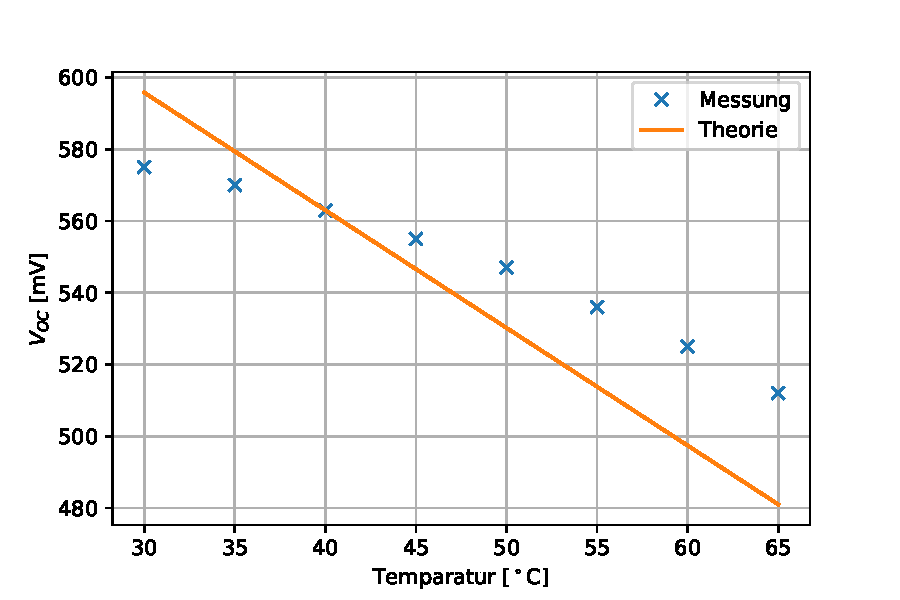
\includegraphics[width=.5\columnwidth]{figs/python/D/ucc.pdf}
        \caption{Temperaturabh\"angigkei von \(\voc\).}
        \label{fig:tempeinf}
\end{figure}

Bei konstanter Intensit\"at sinkt \(\voc\). Das ist zu erwarten, da
mit steigender Temperatur der Diffusionsstrom zunimmt und damit die
Eingbaute Spannung verringert. Dementsprechend sinkt mit \(\voc\) auch
die Effizienz.

Gem\"a\ss{}~\ref{eq:sattigstrom} gilt mit \(E_g \approx
\SI{1.12}{\electronvolt}\) und (siehe~\ref{tab:atemps}) \(T=\SI{305}{\kelvin}\):
\begin{equation}
  \label{eq:is0}
  I_{S0}=I_s\cdot\exp(-\frac{E_g}{k_B\cdot T}) \approx \SI{3e11}{\ampere}
\end{equation}

Damit und ... ergibt sich die in \ref{fig:tempeinf} eingezeichenete
Theoriekurve, welche ohne Betrachtung der Messungenauigkeiten dennoch
ein \"ahnliches verhalten wie die Messwerte zeigt.

Bei diesen Betrachtungen wurde ein konstantes \(\isc\) vorrausgesetzt,
welches auch in guter N\"aherung gegeben
ist. Aus~\ref{fig:tempccurves} folgen f\"ur die Kurzschlussstr\"ome die
in~\ref{tab:isctemps} dargestellten Str\"ome.

\begin{table}[h]
  \centering
  \begin{tabular}{SS}
    \toprule
    {Temperatur [\si{\degreeCelsius}]} & {\(\isc\) [\si{\ampere}]}
    \\
    \midrule
    30 & .031243 \\
    65 & .032597
  \end{tabular}
  \caption{\(\isc\) der anorganischen Zelle A8 bei verschiedenen
    Temperaturen.}
  \label{tab:isctemps}
\end{table}


\begin{figure}[h]\centering
  \begin{subfigure}[b]{1\textwidth}\centering
    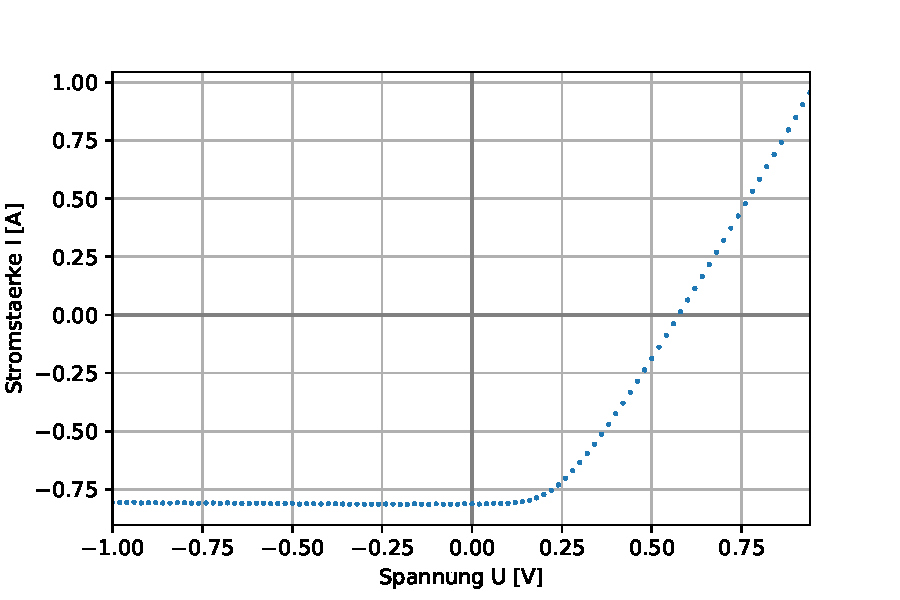
\includegraphics[width=.6\columnwidth]{figs/python/D/30.pdf}
    \caption{Kennlinie bei \SI{30}{\degreeCelsius}}
    \label{diag:t30}
  \end{subfigure}
  \begin{subfigure}[b]{1\textwidth}\centering
    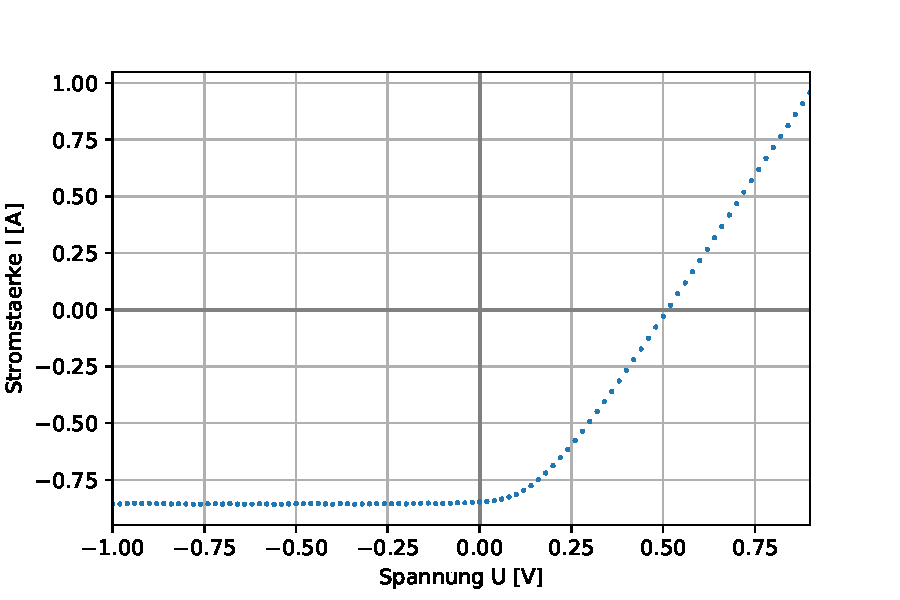
\includegraphics[width=.6\columnwidth]{figs/python/D/65.pdf}
    \caption{Kennlinie bei \SI{65}{\degreeCelsius}}
    \label{diag:t65}
  \end{subfigure}
  \caption{Kennlinien der anorganischen Zelle A8 bei verschiedenen
    Temperaturen.}
  \label{fig:tempccurves}
\end{figure}

Der Photonenstrom bleibt relatic konstant da sich die Lichtintensität
und damit auch die Elektron-Loch Erzeugungsrate nicht \"andert.

\subsection{Winkelabhängigkeit des Stromflusses vom einfallenden Licht}
\label{sec:winkel}

\begin{figure}[H]\centering
        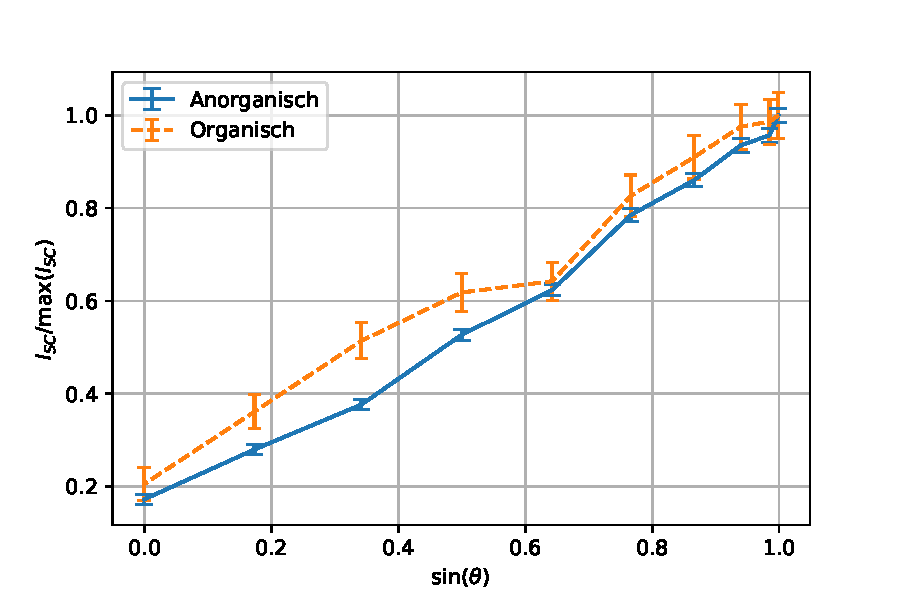
\includegraphics[width=.5\columnwidth]{figs/python/E/relativ.pdf}
        \caption{Winkelabhängigkeit des Stromflusses vom einfallenden Licht}
        \label{fig:winkel}
\end{figure}

Wie in~\ref{fig:winkel} erkennbar gibt es zwischen dem Winkel des einfallenden
Lichtes und dem Stromfluss eine Sinus-Abhängigkeit. Wobei bei einem senkrechten
Lichteinfallswinkel so gut wie kein Strom mehr fließt.
In~\ref{fig:winkel} ist bei \(\sin(\theta) = 0\) zwar noch ein Stromfluss erkennbar,
dieser liegt aber daran, dass das Modul in Richtung der Fenster gedreht wurde und somit,
auch wenn das Wetter am Versuchstag bewölkt war, immer noch genügend Licht auf die beiden
Solarzellen fallen konnte, um einen Stromfluss zu ermöglichen.

\section{Anhang}
\label{sec:anh}

\subsection{Weitere Plots zu C}
\label{sec:plotsc}

\begin{figure}[H]\centering
        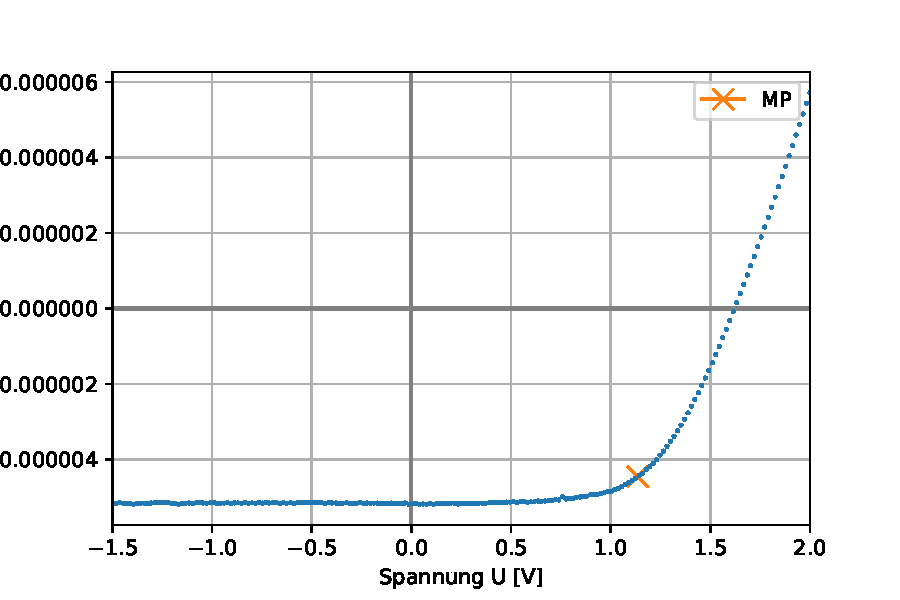
\includegraphics[width=.6\columnwidth]{figs/python/C/3x3_hell.pdf}
        \caption{Hellkennlinie des 6er-Moduls}
        \label{diag:hell6er}
\end{figure}

\begin{figure}[H]\centering
\begin{subfigure}[b]{1\textwidth}\centering
        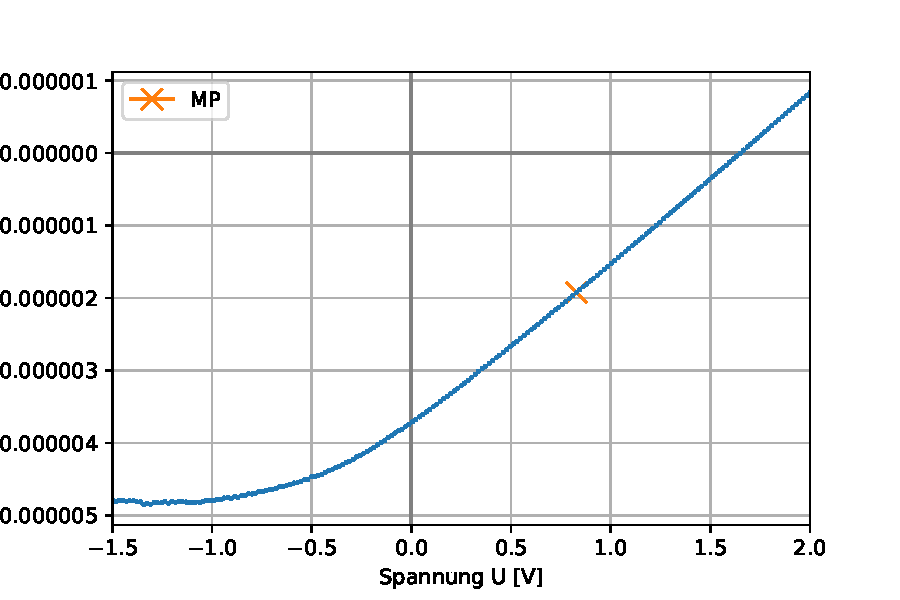
\includegraphics[width=.6\columnwidth]{figs/python/C/3x3_schaltung_2.pdf}
        \caption{Schaltung 1 (vgl.~\ref{fig:schalt1})}
        \label{diag:hellschalt1}
\end{subfigure}
\begin{subfigure}[b]{1\textwidth}\centering
        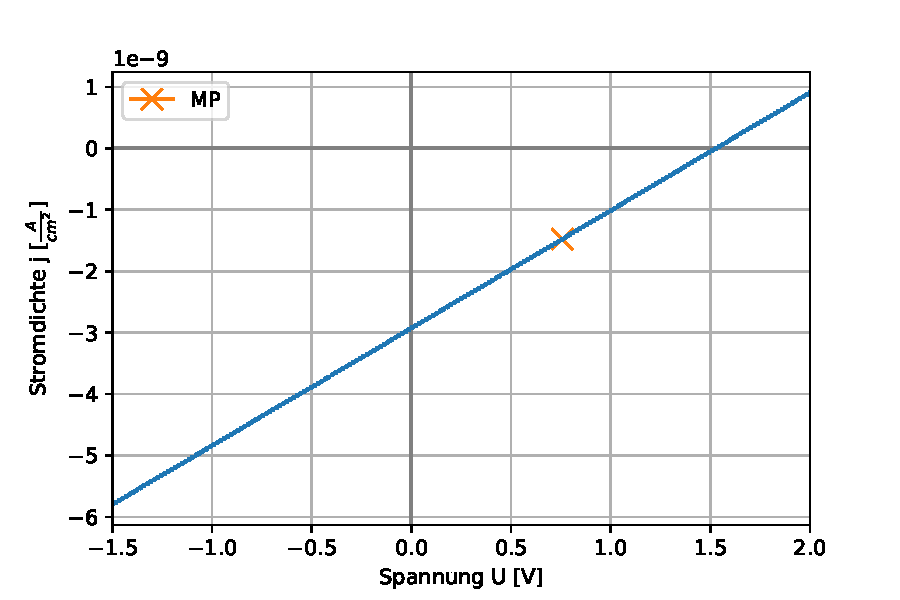
\includegraphics[width=.6\columnwidth]{figs/python/C/3x3_schaltung_3.pdf}
        \caption{Schaltung 2 (vgl.~\ref{fig:schalt2})}
        \label{diag:hellschalt2}
\end{subfigure}
\begin{subfigure}[b]{1\textwidth}\centering
        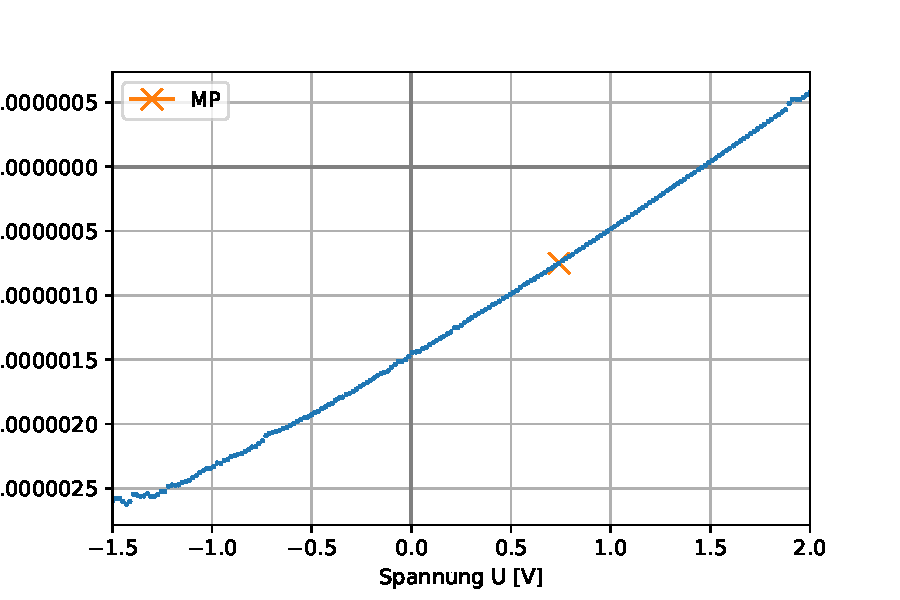
\includegraphics[width=.6\columnwidth]{figs/python/C/3x3_schaltung_4.pdf}
        \caption{Schaltung 3 (vgl.~\ref{fig:schalt3})}
        \label{diag:hellschalt3}
\end{subfigure}
        \caption{Hellkennlinien}
        \label{fig:hellkenn}
\end{figure}

\begin{figure}[H]\centering
        \begin{subfigure}[b]{1\textwidth}\centering

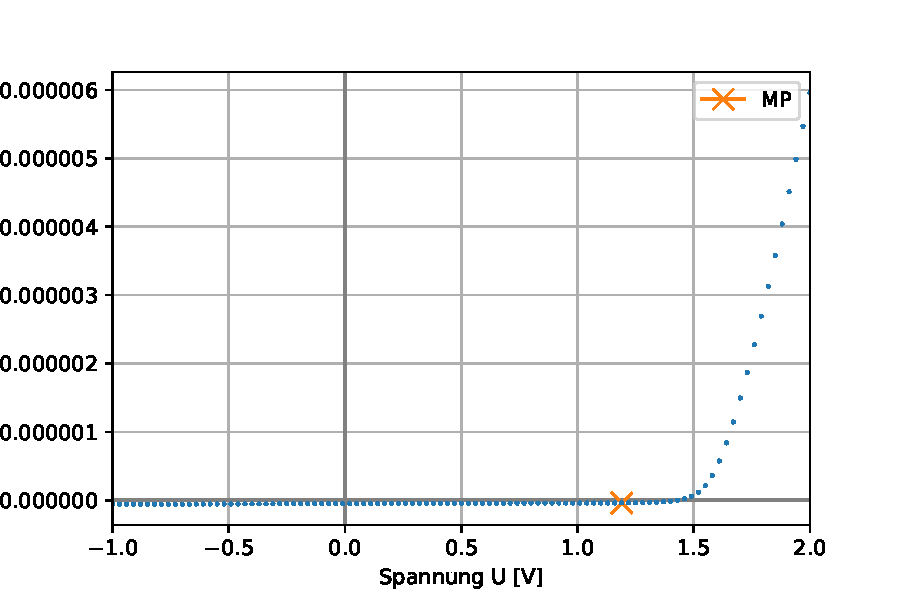
\includegraphics[width=.5\columnwidth]{figs/python/C/3x3_verschattung_1.pdf}
\caption{Verschattung 1 (vgl.~\ref{fig:schatt1})}
\label{diag:verschattung1}
        \end{subfigure}
        \begin{subfigure}[b]{1\textwidth}\centering
                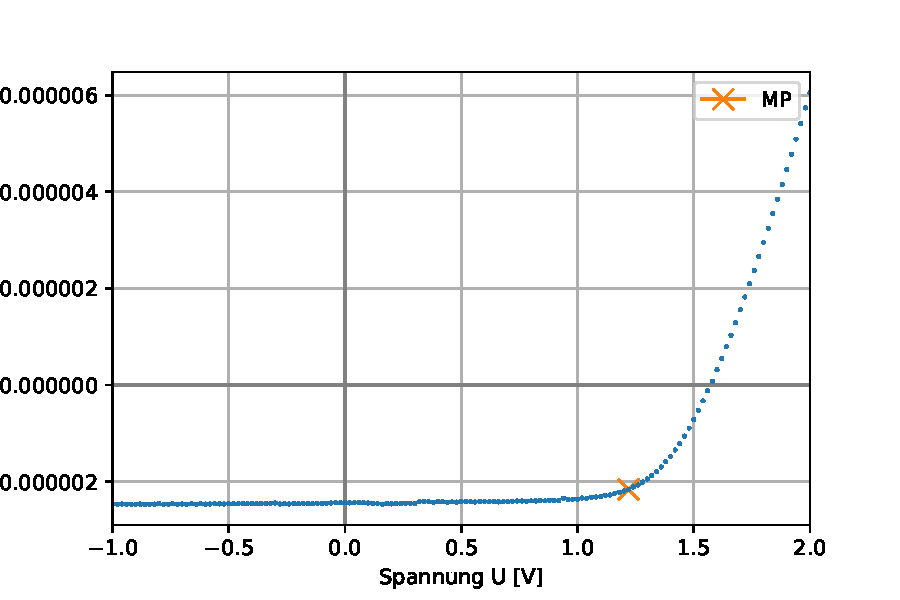
\includegraphics[width=.6\columnwidth]{figs/python/C/3x3_verschattung_2.pdf}
                \caption{Verschattung 2 (vgl.~\ref{fig:schatt2})}
                \label{diag:verschattung2}
        \end{subfigure}
        \begin{subfigure}[b]{1\textwidth}\centering
                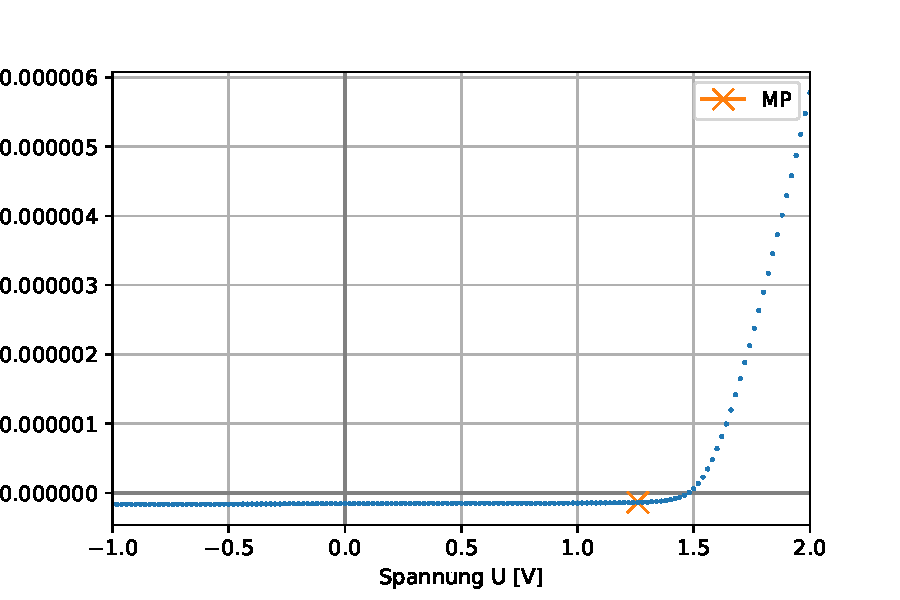
\includegraphics[width=.6\columnwidth]{figs/python/C/3x3_verschattung_3.pdf}
                \caption{Verschattung 3 (vgl.~\ref{fig:schatt3})}
                \label{diag:verschattung3}
        \end{subfigure}
        \caption{Kennlinien für verschiedene Verschattungen}
        \label{fig:verschattung}
\end{figure}

\begin{figure}[H]\centering
        \begin{subfigure}[b]{1\textwidth}\centering
                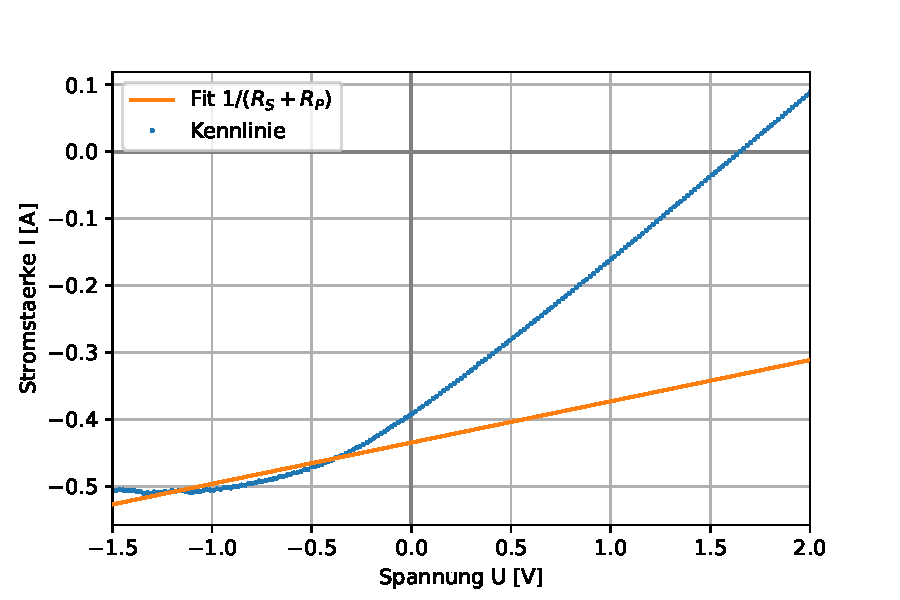
\includegraphics[width=.6\columnwidth]{figs/python/3x3_schaltung_2_rsrp.pdf}
                \caption{Schaltung 1 (vgl.~\ref{fig:schalt1})}
                \label{diag:hellschalt1fit}
        \end{subfigure}
        \begin{subfigure}[b]{1\textwidth}\centering
                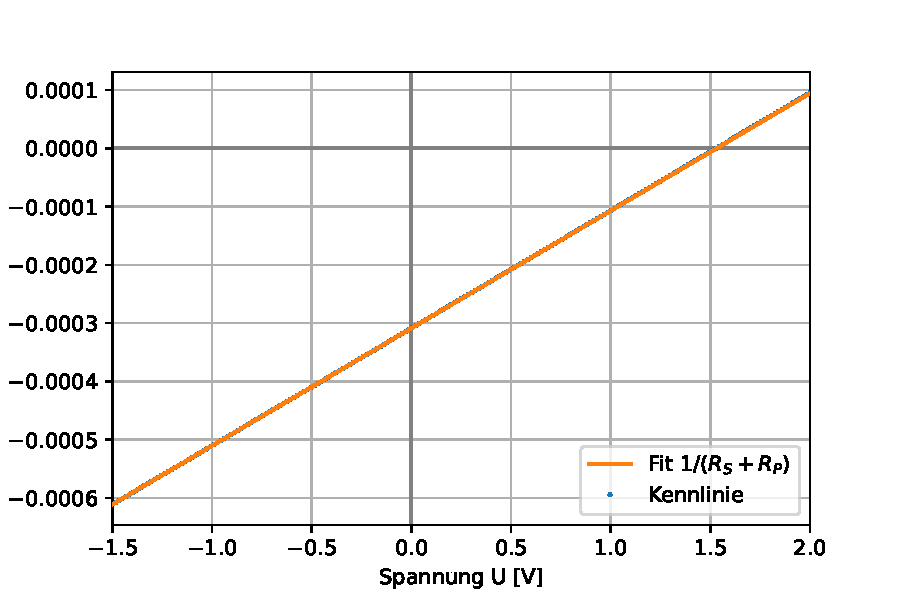
\includegraphics[width=.6\columnwidth]{figs/python/3x3_schaltung_3_rsrp.pdf}
                \caption{Schaltung 2 (vgl.~\ref{fig:schalt2})}
                \label{diag:hellschalt2fit}
        \end{subfigure}
        \begin{subfigure}[b]{1\textwidth}\centering
                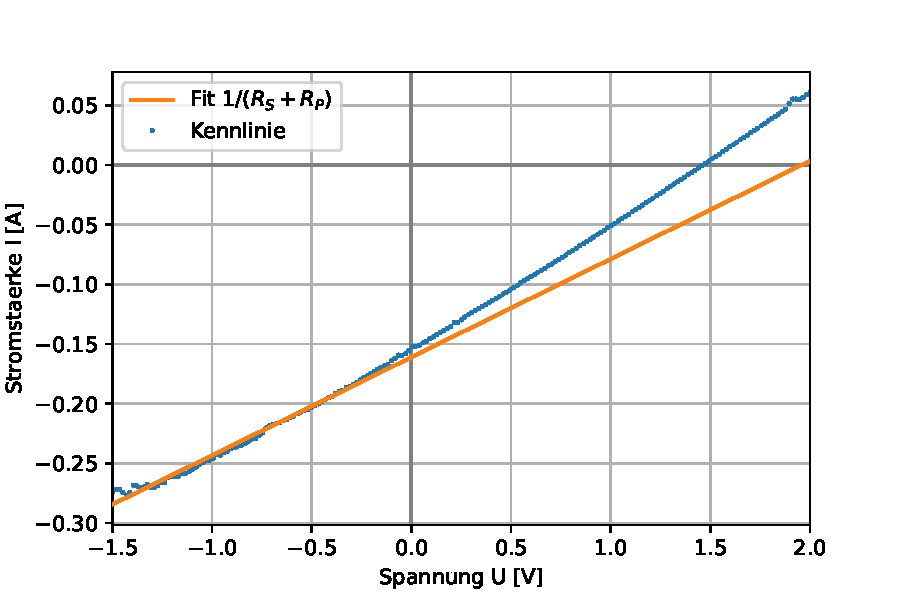
\includegraphics[width=.6\columnwidth]{figs/python/3x3_schaltung_4_rsrp.pdf}
                \caption{Schaltung 3 (vgl.~\ref{fig:schalt3})}
                \label{diag:hellschalt3fit}
        \end{subfigure}
        \caption{Hellkennlinien mit Fits f\"ur den Parallelwiderstand}
        \label{fig:hellkennfit}
\end{figure}


\begin{figure}[H]\centering
        \begin{subfigure}[b]{1\textwidth}\centering
                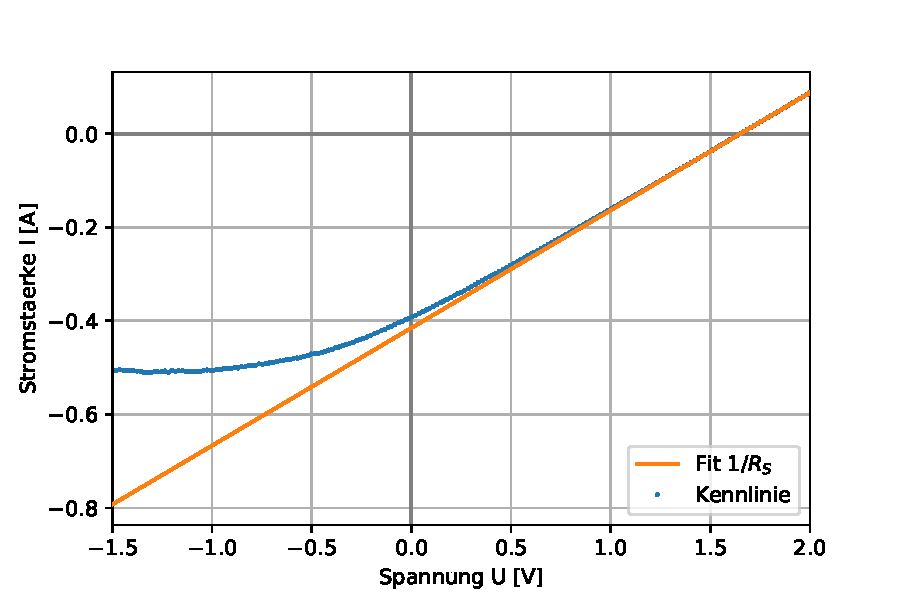
\includegraphics[width=.6\columnwidth]{figs/python/3x3_schaltung_2_rs.pdf}
                \caption{Schaltung 1 (vgl.~\ref{fig:schalt1})}
                \label{diag:hellschalt1fit1}
        \end{subfigure}
        \begin{subfigure}[b]{1\textwidth}\centering
                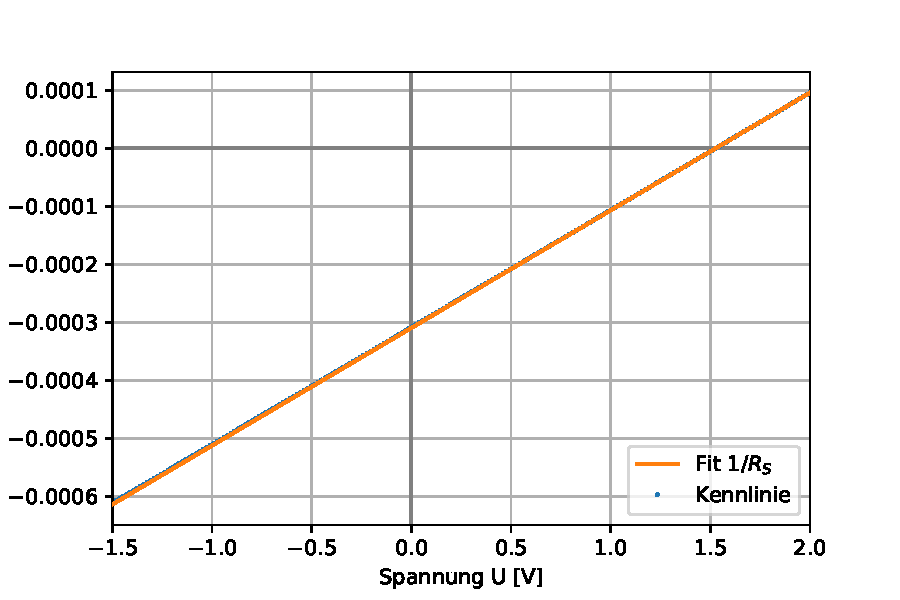
\includegraphics[width=.6\columnwidth]{figs/python/3x3_schaltung_3_rs.pdf}
                \caption{Schaltung 2 (vgl.~\ref{fig:schalt2})}
                \label{diag:hellschalt2fit1}
        \end{subfigure}
        \begin{subfigure}[b]{1\textwidth}\centering
                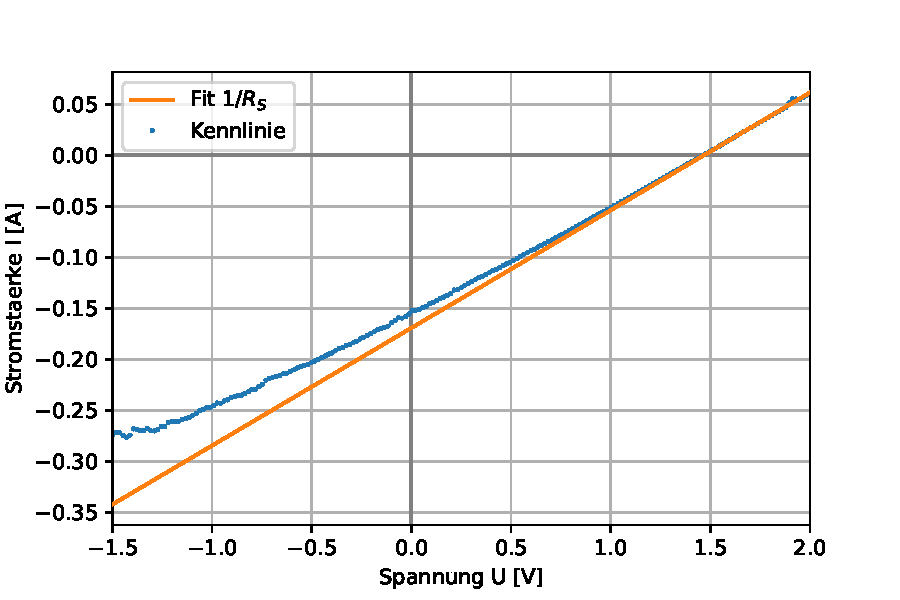
\includegraphics[width=.6\columnwidth]{figs/python/3x3_schaltung_4_rs.pdf}
                \caption{Schaltung 3 (vgl.~\ref{fig:schalt3})}
                \label{diag:hellschalt3fit1}
        \end{subfigure}
        \caption{Hellkennlinien mit Fits f\"ur den Serienwiderstand}
        \label{fig:hellkennfit1}
\end{figure}

\begin{figure}[H]\centering
        \begin{subfigure}[b]{1\textwidth}\centering
                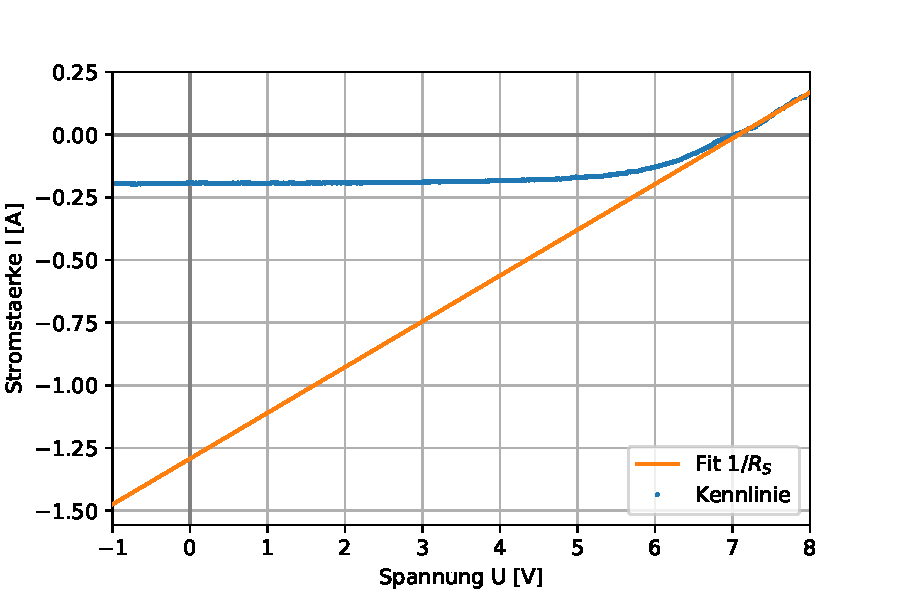
\includegraphics[width=.45\columnwidth]{figs/python/huge_hell_rs.pdf}
                \caption{13er Modul ohne Verbraucher mit \(R_S\)-Fit}
                \label{diag:hugehellrs}
        \end{subfigure}
\begin{subfigure}[b]{1\textwidth}\centering
        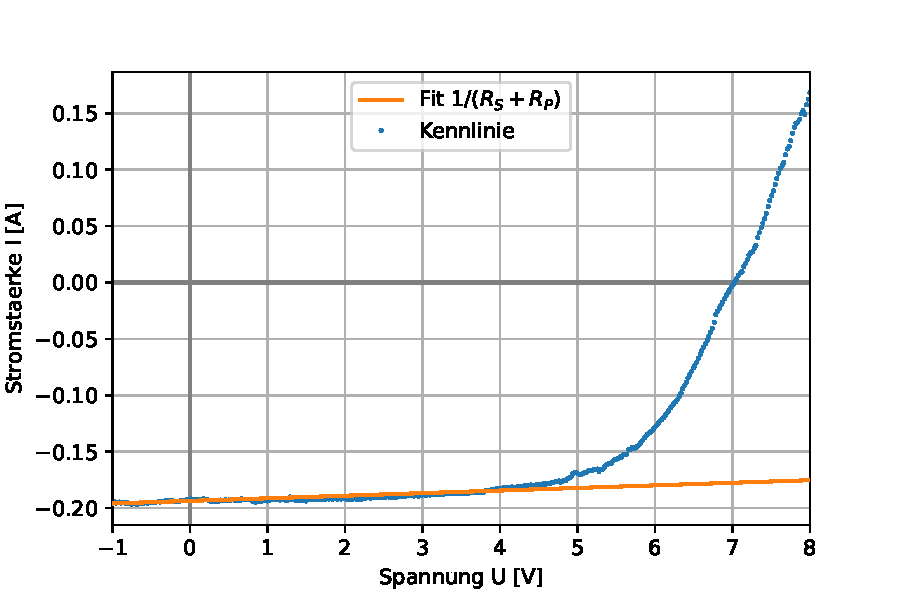
\includegraphics[width=.45\columnwidth]{figs/python/huge_hell_rsrp.pdf}
        \caption{13er Modul ohne Verbraucher mit \(R_S\)- und \(R_P\)-Fit}
        \label{diag:hugehellrsrp}
\end{subfigure}
        \begin{subfigure}[b]{1\textwidth}\centering
                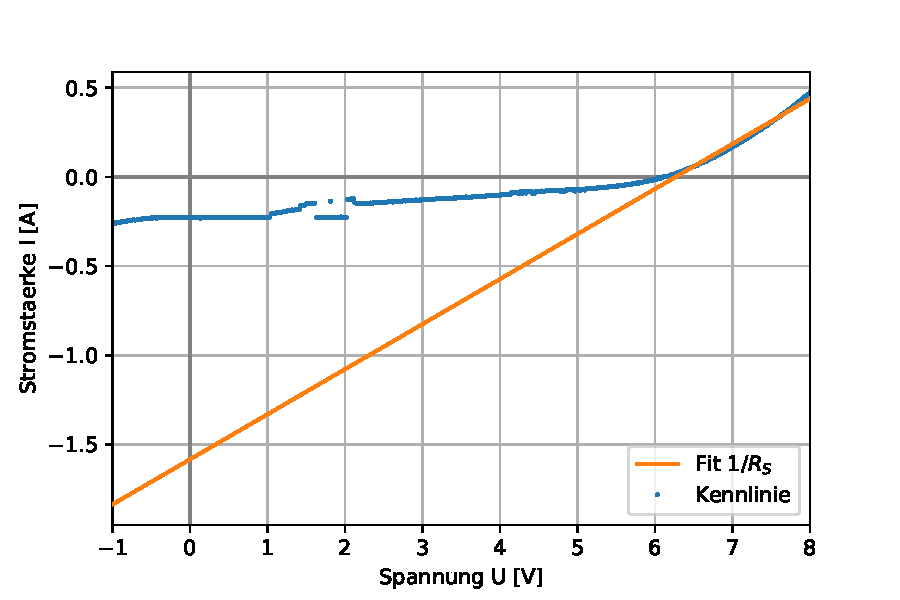
\includegraphics[width=.45\columnwidth]{figs/python/huge_verbraucher_rs.pdf}
                \caption{13er Modul mit Verbraucher mit \(R_S\)-Fit}
                \label{diag:hugeverbrrs}
        \end{subfigure}
\begin{subfigure}[b]{1\textwidth}\centering
        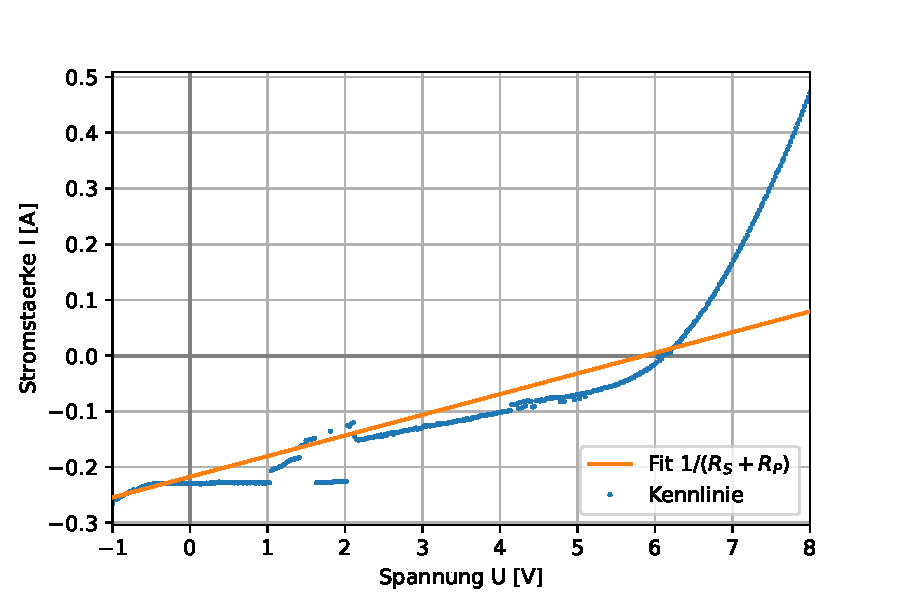
\includegraphics[width=.45\columnwidth]{figs/python/huge_verbraucher_rsrp.pdf}
        \caption{13er Modul mit Verbraucher mit \(R_S\)- und \(R_P\)-Fit}
        \label{diag:hugeverbrrsrp}
\end{subfigure}
        \caption{Kennlinien des 13er Solarmoduls}
        \label{fig:huge}
\end{figure}

\subsection{Messwerte zu D}

\begin{table}[H]
        \centering
        \begin{tabular}{l|l}
                \toprule
                \(T [\si{\degreeCelsius}]\) & \(\voc [\si{\milli\volt}]\)\\
                \midrule
                35 & 570 \\
                40 & 563 \\
                45 & 555 \\
                50 & 547 \\
                55 & 536 \\
                60 & 525 \\
                65 & 512
        \end{tabular}
        \caption{Leerlaufspannung in Abhängigkeit zur Temperatur}
        \label{tab:messd}
\end{table}

\subsection{Messwerte zu E}

\begin{table}[H]
        \centering
        \begin{tabular}{l|l|l}
                \toprule
                \(\text{Winkel} [^\circ]\) & \(I_{org} [\si{\milli\ampere}]\) &\(I_{anorg} [\si{\ampere}]\) \\
                \midrule
                87 & 0.288 & 0.93 \\
                80 & 0.284 & 0.89 \\
                70 & 0.281 & 0.87 \\
                60 & 0.262 & 0.80 \\
                50 & 0.238 & 0.73 \\
                40 & 0.195 & 0.59 \\
                30 & 0.177 & 0.49 \\
                20 & 0.148 & 0.35 \\
                10 & 0.104 & 0.26 \\
                0 & 0.059 & 0.16 \\
        \end{tabular}
        \caption{Kurzschlussstrom in Abhängigkeit des Winkels des einfallenden Lichts}
        \label{tab:messe}
\end{table}

\section{Literatur}

\label{sec:literatur}

\printbibliography
\end{document}
